\documentclass[	runningheads,
				%deutsch, % Tell llncs that the keywords should be in german
				%german,  % Needed for the \ifgerman-command
				a4paper]{llncs}

\usepackage{url}
\usepackage{graphicx}
\usepackage{amssymb}
\usepackage{hyperref}

% Support for special characters like "Umlaute"
\usepackage[utf8]{inputenc}

\usepackage[english]{babel}

\usepackage{glossaries}
\usepackage{caption}
\usepackage{subcaption}

\makeglossaries

\loadglsentries{glossary}
%*********************************************************************%
% META                                                                %
%*********************************************************************%
\newcommand{\university}{Saarland University}
\newcommand{\school}{Saarland Informatics Campus}
\newcommand{\thetitle}{Seminar: Systems Benchmarking}
\newcommand{\shorttitle}{Systems Benchmarking}
\newcommand{\thedate}{\today{}}
\newcommand{\thegermandate}{15. April}

\newcommand{\theforename}{Lukas}
\newcommand{\thesurname}{Abelt}

% Advisors
	\newcommand{\advisor}{Advisors}
	\newcommand{\advisors}{Prof. Sven Apel, \\ Christian Hechtl}

% Title for the seminar
\newcommand{\theseminartitle}{"Performance Measurements Before Releases vs. Each Commits"}
%\newcommand{\theseminartitle}{"Using Benchmarking in Productive Development Systems -- Opportunities and Challenges"}

%*********************************************************************%
% THE DOCUMENT                                                        %
%*********************************************************************%

\begin{document}
	%*********************************************************************%
	% TITLE                                                               %
	%*********************************************************************%
	
	% Arabic page numbering
	\mainmatter 
		
	% Title including a subtitle for the name of the seminar
	\title{\theseminartitle \\ \small \thetitle}
	
	% (Optional) In the case that the initial title is too long, the short title will be used
	%\titlerunning{Hauptseminar: Human and Social Factors in Software Engineering}
	
	\author{\theforename\ \thesurname \small \\ \ \\ \advisor : \ \advisors}
	
	% (Optional) This will appear near the page number
	\authorrunning{\shorttitle}
	
	\institute{\school ,\\ \university}
	
	\maketitle
	
	%*********************************************************************%
	% CONTENT                                                             %
	%*********************************************************************%

% General Structure
	% 1. Introduction and Motivation
	% 2. General Definitions
	%		2.1 What is a Benchmark
	%		2.2 What is a continuous Benchmark
	% 3. Experiment
	%		3.1 Experiment Idea&Goals
	%		3.2 Setup
	%		3.3 Evaluation
	%	4. 

	% Introduction
\section{Introduction}
Over the past years system benchmarks have become more prominent in a variety of contexts and use cases. As a result more benchmarking tools became available that are used in both commercial systems and are widely adopted for academic purposes.

This paper gives an overview of the general concepts of system benchmarks and describes how classical benchmarking approaches can be used and extended to integrate them into the standard development process of software. Specifically, it will outline how benchmarks can be used to swiftly detect and react to performance changes throughout the development process. In order to achieve this the paper will describe and use the concepts of change point detection. This paper will outline and analyse the methodology and opportunities of such approaches while taking a careful look at the challenges that may arise due to this.

To support and evaluate the claims, this paper includes a practical experiment that will serve as a basis to compare two benchmarking approaches on a piece of well known, open-source software.

\section{System Benchmarks}
\label{sec:benchmarking}
The term "Benchmark" is a broad term that can be interpreted and defined in many different ways depending on the context and application domain. This chapter gives a general definition of "Benchmarking" how it will use it throughout this paper.

\subsection{Definition}
\label{ssec:bench_definition}
The term "Benchmark" is used in a variety of different domains and, according to the Standard Specialization Evaluation Corporation, historically stems from a physical marking that was used as a reference point on a workbench to check the length of the produced pieces\footnote{SPEC Glossary: \url{https://www.spec.org/spec/glossary/\#benchmark}}. However throughout this paper we are only interested in system benchmarks within the context of software systems and will therefore also refer to the definition of a benchmark as given by Kounev et al.: "a tool coupled with a methodology for the evaluation and comparison of systems or components with respect to specific characteristics, such as performance, reliability or security." (\cite{Kounev} p. 4). As already given from this definition benchmarks can serve as an evaluation for different characteristics. We will more closely look at these in \autoref{ssec:bench_classification}. Throughout this paper we will also mostly refer to the "system or component" that is being benchmarked as the \gls{sut}.

\subsection{Classification of Benchmarks}
\label{ssec:bench_classification}
Benchmarks can be classified in a variety of different means. In this section we will give a small overview of the different types of benchmarks there are with respect to the two following questions:
\begin{enumerate}
	\item What overall goal does a benchmark serve?
	\item What qualities are evaluated by an benchmark?
	\item How can a benchmark be performed (Benchmarking strategies)
\end{enumerate}

In the broadest sense, benchmarks can be divided into competitive and non-competitive benchmarks. The main motivation of competitive benchmarks is hereby the development of standardized quality criteria that can be used to compare different systems. Certain sources also emphasize this importance on the competitiveness by providing a more detailed definition of the term benchmark, i.e. "a standard tool for competitive evaluation and comparison of competitive systems" (\cite{kistowski2015} p. 333).

For non-competitive benchmarks Kounev et al. Further distinguish between the two categories of "rating tools" and "research benchmark". Rating tools can serve multiple purposes: Either as a component of an development and system improvement process, as a baseline for regulatory programmes or to serve as common benchmark for research. Research benchmarks on the other hand commonly refer to tools and workloads that may be used for in-depth evaluation of research results, prototypes or productive systems. Based on these descriptions it becomes apparent that there sometimes might be no clear distinction between a rating tool and a research benchmark and the terminology is often determined by the evaluating party (See \cite{Kounev} p. 4).

Regardless of the competitiveness, or lack thereof, of a benchmark the key metrics that are evaluated are often similar or even identical. While historically the main metrics of importance were e.g. security, system reliability and energy efficiency, modern benchmarks also try to cover much more aspects of a software. According to Kounev et al. quality metrics of modern benchmarks are usually(\cite{Kounev} p. 6 f):
\begin{itemize}
	\item Performance
	\item Scalability
	\item	Energy Efficiency
	\item Reliability
\end{itemize}

%\paragraph{Performance} The term Performance itself can be interpreted in many different means. For this paper, we will focus on one of the most basic interpretations: The amount of work done compared to the time and resources used. A much more in-depth explanation of different performance measures is given by Kounev et al. (See \cite{Kounev} p. 49 ff)

%\paragraph{Scalability} TODO Definition needed

%\paragraph{Energy Efficiency} TODO Definition needed

%\paragraph{Reliability} TODO Definition needed

In terms of benchmarking strategies three general approaches can be distinguished:
\begin{enumerate}
	\item Fixed-Time Benchmarks
	\item Fixed-Work Benchmarks
	\item Variable Time- and Work-Benchmarks
\end{enumerate}

All of these offer there own benefits, drawbacks and specific use-cases. These are discussed in detail by Kounev et al.(\cite{Kounev} p. 9ff)

%When it comes to benchmarking strategies two approaches are most prominent: Fixed-Time and Fixed-Work benchmarks. A Fixed-Work Benchmark here describes the most intuitive approach for benchmarking: We fix a specified amount of work $W_i$ and measure the required time $T_i$ that is required to fulfil this work.

%While Fixed-Work benchmarks are easy to understand and implement, it introduces an implicit performance bottleneck that is also known as \textit{Amdahl's Law}. It states that the maximum possible performance improvement that can be achieved in Fixed-Work Benchmarks is upper-bounded by the fraction of work that is performed by the component that is being improved (See \cite{Kounev} p. 9f).

%In Fixed-Time benchmarks, instead of fixing the amount of work $W_i$, the time $T_i$ is bound and the amount of work finished in this time is measured as a metric. As opposed to Fixed-Work Benchmarks the Fixed-Time Benchmarks do not suffer the issue of an upper-bounded maximum improvement as for every improvement, the reduced time can be used to process further work units (See \cite{Kounev} p. 11).

%Additionally there are also further approaches that does not employ fixed time or work at all, but rather employ variable-time and -work characteristics. For this case the metric is a function of the time $T$ and the work $W$. While this technique provides maximum flexibility, this approach is not suitable for all types of benchmarks (See \cite{Kounev} p. 12)

\subsection{Evaluating Benchmarks}
\label{ssec:eval_bm}
Apart from the metrics that evaluate the result of a benchmark, there are also several attributes that are important to evaluate the quality of the benchmark itself. The designer of a benchmark should always take these attributes into consideration when creating a benchmark. As described by Skadron et al. it is not possible to create a single benchmark that covers all these attributes perfectly. Therefore one either has to create multiple benchmarks that complement each others weaknesses or choose to sacrifice one of these attributes over the other (\cite{Skadron2003} p. 32f).

Over the years, researchers and industry associates alike have defined several criteria that are considered desirable by modern standards. Often the exact terminology of these criteria differs based on authors and the specific application domain, however the concepts in general are similar. Kounev at al. list five core criteria that are generally of interest(\cite{Kounev} p. 13f). A much more in depth discussion of these criteria was performed by Kistowski et al. (See \cite{kistowski2015})
\begin{itemize}
	\item Relevance
	\item Reproducibility
	\item Fairness
	\item Verifiability
	\item Usability
\end{itemize}
%\paragraph{Relevance} For a benchmark to be meaningful it is important that it, at least to a certain extent, reproduces some scenarios with real world application. This is what the "Relevance" of a benchmark refers to. It tries to define how relevant the produced information is to a potential user of a software. According to Kistowski et al. this makes it "perhaps the most important characteristic" (\cite{kistowski2015} p. 334). However the relevance of a benchmark may also limits the benchmarks applicability meaning, that a highly relevant benchmark for a specific system or component might only narrow applicability while benchmarks with a broad applicability will have a lower relevance but for a wider selection of applications. Kistowski et al. further elaborate on this with specific examples (\cite{kistowski2015} p. 334f)

%\paragraph{Reproducibility} Reproducibility ensures that it is possible for a third party to produce ideally the same results for a given test environment. Reproducibility covers both the consistency between multiple runs on the same system as well as creating the same results on another environment with a semantically equivalent configuration. 

%However, with modern hard- and software systems, optimal reproducibility has become challenging. For both hard- and software there are several factors that induce variability. From a hardware side things such as the physical disc layout or network connections may affect benchmarking results. For software systems the causes for variability stem from various different sources. from a low-level perspective, things such as thread scheduling can influence the benchmark results. From a higher level perspective a benchmark has to consider the configurability of a software system itself. Modern software systems often offer lots of different configuration options which can be used to create a tailor made system-variant. En- or disabling a specific feature might heavily influence the performance of a benchmark.

%According to Huppler, an ideal benchmark result should be definable as a function of a hard- and software configuration (See \cite{huppler2009} p. 335). However for real-world applications, modelling such a function is far too complex which requires the benchmark designer to try to model reproducibility in other ways. In the end the reproducibility of a benchmark is heavily dependent on the ability to reproduce the benchmarking environment that was used to create this specific benchmark. 

%\paragraph{Fairness} TODO: Short explanation
%\paragraph{Verifiability} TODO: Short explanation
%\paragraph{Usability} TODO: Short explanation

\section{Using Benchmarks to Detect Performance Changes}
\label{sec:bench_perf_changes}
	This section will discuss how benchmarks can be used during software development to detect performance changes.
	
	\subsection{Opportunities}
	\label{ssec:bench_perf_oppo}
	While benchmarks as a stand-alone tooling are already a useful tool to compare the performance of different systems in order to, for example, select a specific system for a given task it also offers different opportunities. One of these opportunities is to use benchmarking as a tool that is closely integrated into the development cycle in order to evaluate the systems performance throughout the development.

	There are different goals to consider when integrating benchmarking into the development process. Most prominently benchmarking can be used as a quality measure to evaluate a software systems performance. Due to the increasing complexity in modern software systems it is often not possible to foresee the impact of even a small change to the performance of a complex software system (See \cite{grambow2019} p. 1, \cite{daly2021} p. 1). 
	
	As a result if not including any performance evaluation might lead to performance regressions being shipped in a stable release to customers and users. Therefore using benchmarks throughout the development process can ensure to detect performance changes and allows to fix them before they are being released (See \cite{daly2021} p. 1). 

	Additionally employing benchmark on a regular basis also opens the window of opportunity for many other improvements if the corresponding infrastructure is setup accordingly. Daly describes in great detail how this was achieved for the MongoDB infrastructure in \cite{daly2021}. In summary the following have been observed:
	\begin{itemize}
		\item Increased productivity of the developers
		\item Reduced noise on the performance data
		\item Improved Comparison of arbitrary results
		\item An increased amount of performance improvements
	\end{itemize}

	For this chapter we want to focus on two main questions; How can performance benchmarking be used to:
	\begin{enumerate}
		\item Quickly and reliably detect performance changes?
		\item Compare arbitrary development states?
	\end{enumerate}

	The underlying overall question however is, when or how often, one needs to perform a benchmark in order to sufficiently answer these questions. For this two approaches will be compared in the following subsections:
	\begin{enumerate}
		\item Benchmarking Before Publishing a new Release
		\item Benchmarking Every Commit -- Which we will refer to a \textit{Continuous Benchmarking}
	\end{enumerate}

	\subsection{Benchmarking Before Releases}
	\label{ssec:bench_rel}
	The most intuitive approach to ensure the performance of a software system throughout the release history is quite simple: Based on the requirements imposed by either a customer or internal quality assurance one defines certain performance threshold that the software needs to fulfil. Based on these quality criteria the development team can build a benchmark that can check these attributes.

	Once the software is nearing a new release and e.g. a new \textit{Release Candidate} is created internally, the development team can use this benchmark to evaluate whether the candidate introduces a performance regression or if it is fit for a release. There are several benefits of this approach; First of all, it does not necessarily requires an automated performance testing infrastructure but rather can be executed and evaluated manually be the development team. 

	However this approach also bears various challenges that need to be considered in the development of modern software systems. Daly describes two main challenges that arose when using this approach in the development of MongoDB: Firstly it is possible that test from the last release cycle are simply not reproducible with the current software, secondly identifying the exact change that introduced a performance regression poses challenging (\cite{daly2021} p. 1f).

	Both of these challenges are heavily influenced by the length of software release cycles and the resulting amount of commits throughout one cycle. As an example one can take a look at a few open-source repositories. The C++ test framework \textit{googletest} (\cite{gtest}) by Google with it's most recent release (\textit{1.11.0}) in June 2021, while the last release before that (\textit{1.10.0}) was released in October 2019. During this period of 28 months roughly 700 commits have been added to the repository. Similarly for the C implementation of the \texttt{lz4} compression algorithm that can be found on GitHub (\cite{gitlz4}) in the 15 months between the two most recent releases about 250 commits have been added to the code.

	This can also be observed in commercially used software such as MongoDB which reported about 5500 commits to their code throughout the 2019/2020 release cycle averaging to just about 15 commits per day (\cite{daly2021} p. 2). If the only benchmarking data available is these from the two release candidates this results in an extensive additional overhead to retroactively reconstruct the cause of the root cause. Additionally when only evaluating the performance before release candidates as an affect one would also only detect a performance change at that point. However generally software aims to detect performance defects as soon as possible. 

	One additional dimension that has to be considered is the aspect of configurability. In modern software systems there are often configuration options available which allows to en- and disable certain features to create a tailor-made system variant. However, this additional layer of complexity adds further challenges to benchmarking and change detection. As already very few configuration options lead to an combinatorial explosion of the possible system variants which makes it unfeasible to benchmark all of them(See \cite{apel2020} p. 1).

	\subsection{Continuous Benchmarking}
In this section a technique that will further be referred to as \textit{Continuous Benchmarking} will be elaborated further. First the motivation of this approach will be discussed to give a working definition. Secondly a selection of possible continuous benchmarking strategies will be outlined. Lastly the possible benefits and potential challenges will be showcased and weighted to give an assessment of using such a technique.

	\subsubsection{Definition}
	As previously discussed in \autoref{ssec:bench_rel} benchmarking only before releases introduces several challenges. The general motivation of continuous benchmarking is to address these by, simply said, generally adding more data points to evaluate. These added data points can then be used for a more detailed analysis of the systems performance over time. The general idea is similar to those used in \gls{ci} and \gls{cd}. By running tests and releases more frequently, often after every commit, these methods aim to shorten release cycles. \gls{cb} however, is a term and methodology that seems not yet commonly defined in academia.

	We will therefore introduce the following (working) definition for our approach to continuous benchmarking in this paper:
	\paragraph{Continuous Benchmarking} -- A Systems Benchmarking integrated into a Continuous Integration pipeline which allows to track a (software) systems performance throughout the development process.

	\paragraph{}As for any benchmark also \gls{cb} should only be run against a correctly working software. Therefore if integrated into a continuous integration pipeline, \gls{cb} should be among the last steps such that the correct functionality of the software is already ensured by the \gls{cd} tests beforehand (See \cite{grambow2019} p. 2).

	Similar to \gls{cd} approaches in \gls{cb} the question also arises when to run the \gls{cb}. For \gls{cd}, optimally all tests and operations should be performed after every commit. However in practice this might not always be feasible due to the amount of tests and the associated compute time with that which is why complex software systems often already use a multi-tiered approach to \gls{cb}. A similar question arises when deciding on when to run \gls{cb}. Running benchmarks after every commit can pose challenges which will be further evaluated in the following section. However for this paper our main focus will not be on when to run \gls{cb} but rather how the data produced by a \gls{cb} can be used to detect performance changes.

		\subsubsection{Opportunities and Challenges}
		\label{sssec:cd_challenges}

		Using \gls{cb} opens up several opportunities for improvements to the development process of software. First of all it gives a regular overview of a software systems performance. However the usability of these results is also heavily dependent on the quality of the testbed. Especially the use of cloud infrastructure can introduce additional noise to the performance of a system. As has been shown by Daly and Ingo in \cite{daly2019} reducing the noise in such a scenario is a heavily application specific task that can take several weeks of investigating the systems behavior.

	Running performance benchmarks more frequently naturally also enables to detect performance changes more quickly. As a result it also makes it easier to isolate the cause of the change as there may only be fa few commits between the two benchmarks. However again the comparability of these results heavily depends how and if we can take into account the testbed's noise accordingly as to not erroneously flag outliers from noise as actual performance changes. In \cite{daly2021} Daly proposed a technique called \textit{canary testing} to counter these issues. However, in their evaluation canary testing was not viable in their productive system and resulted in more cost than benefit (See \cite{daly2021} p. 6f).

	Another point to consider when using \gls{cb} is the additional data that will inherently get produced. Especially for modern software systems there is not only a single benchmark that is of interest but rather multiple benchmarks with for example different system configurations or workloads. Therefore as Daly et al. and Grambow et al. conclude in their works that manually reviewing the performance data for \gls{cb} is not feasible(See \cite{daly2020} p. 2, \cite{grambow2019} p. 5). As a result, to assist in \gls{cb} and especially in detecting performance changes, automated approaches and toolings are required to pre-process this data and possibly detect performance changes automatically. Approaches for such tools have been described by Daly et al. (\cite{daly2020} p. 2, \cite{daly2021} p. 2ff) and Grambow et al.(\cite{grambow2019}). One of the techniques commonly referred to in this context is change point detection which will be covered in a little more detail in \autoref{sec:cp_detection}.

	Lastly setting up the benchmark itself needs to be considered. There might not be standard tooling available for the specific software or benchmark one wants to perform, therefore additional effort may be required to build a benchmark first (See \cite{grambow2019} p. 5). However the same effort has to be done when performing benchmarks manually so it is not a problem that is unique to \gls{cb}. What is an additional challenge for \gls{cb} however, is the increased amount of hardware and computing time required. In order to produce relevant results a benchmark should ideally reproduce a production-like environment. Therefore for complex software system an individual benchmark is considered to be run for at least 20 minutes (\cite{grambow2019} p. 2). If we take into consideration the amount of commits to modern software already outlined in \autoref{ssec:bench_rel}, most likely additional infrastructure will be required if benchmarking is integrated as an automated process. 

	\section{Change Point Detection}
	\label{sec:cp_detection}
	This chapter will give a brief introduction into a technique from signal processing known as \textit{Change Point Detection}. It will briefly introduce the term Change point and it's distinction from outliers and introduce one specific change point detection algorithm. 
	
	\subsection{Definition \& Distinction}
	\label{ssec:cp_distinction}
	The most commonly domain where the term "Change Point" and "Change Point Detection" are commonly used is the one of signal processing. Literature suggest several different definitions of what a change point is.  According to Aminikhanghahi and Cook: "A change point represents a transition between different states in a process that generates the time series data."(\cite{Samaneh2016} p. 4). It is important to understand the fundamental difference between a change point and an outlier in a time series. The NIST\footnote{National Institute of Standards and Technology} Engineering Statistics Handbook defines an outlier as "an observation that lies an abnormal distance from other values in a random sample from a population." (\cite{nist}, part 7.1.6). 

	\begin{figure}[ht!]
		\centering
		\begin{subfigure}[b]{0.45\textwidth}
			\centering
			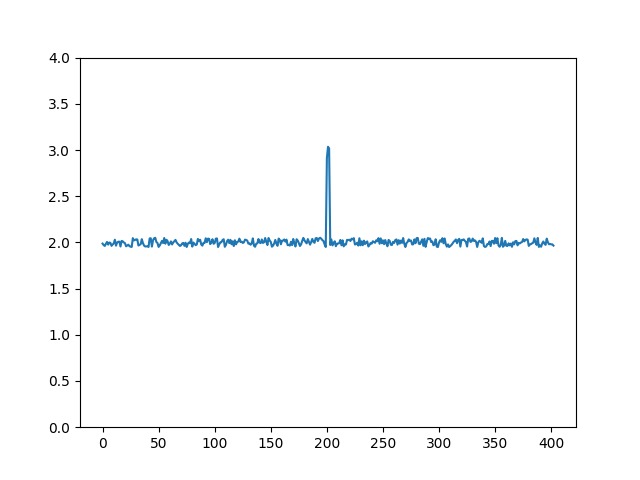
\includegraphics[width=\textwidth]{graph/outlier}
			\caption{Visualization of an outlier}
		\end{subfigure}
		\begin{subfigure}[b]{0.45\textwidth}
			\centering
			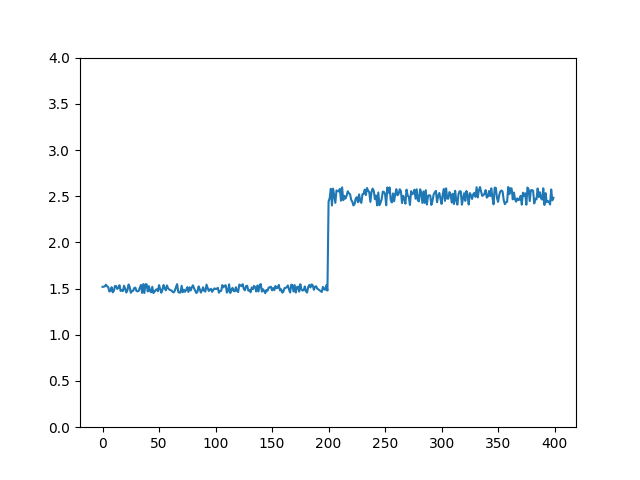
\includegraphics[width=\textwidth]{graph/changepoint}
			\caption{Visualization of a change point}
		\end{subfigure}
		\caption{Visual difference of an outlier and a change point}
		\label{fig:outlier_cp}
	\end{figure}

	In other words, a change point indicates that the overall underlying signal undergoes a noticeable change after that point, while an outlier is only a temporary effect that generally does not persist. \autoref{fig:outlier_cp} shows a visualization of this distinction.

	The challenge of finding such change points is commonly referred to as "Change Point Detection" and is defined by Aminikhanghahi and Cook as "the problem of finding abrupt changes in data when a property of the time series changes" (\cite{Samaneh2016}). In the domain of (continuous) benchmarking, change point detection can be used as a tool to determine points at which a performance regression (or improvement) occurs. With this regard, the performance of a system throughout different commits can be interpreted as a series of time-ordered series, which represents the underlying signal that is analyzed by a change point detection algorithm (See \cite{daly2020} p. 69)

	\subsection{E-Divisive Means}
	\label{ssec:cp_edivisive}
	One algorithm for detecting change points is the E-Divisive Means algorithm. In contrast to other change point detection algorithms it offers a few benefits described by Daly et al. (See \cite{daly2020} p. 69):
	
	\begin{itemize}
		\item No distributional assumptions required
		\item Can identify multiple change points using recursion
		\item Does not require training data
	\end{itemize}

	The algorithm is based on hierarchically dividing the given time-series into multiple clusters. The recursive approach can be summarized in three steps:
	\begin{enumerate}
		\item For each point in the time series calculate a statistic $\hat{Q}$
		\item Select the largest $\hat{Q}$ as the next change point
		\item This divides the time series into two new clusters
	\end{enumerate}

	The termination of the algorithm for a specific cluster is determined by repeating the above steps on a random permutation of the input cluster data. If then the highest $\hat{Q}$ value does not significantly changes it is likely that the series does not contain a relevant change point.

	Within this paper the readily available python package implemented by engineers of MongoDB will be used(\cite{gitmongo}). A broad overview of the algorithm that includes the exact calculation of $\hat{Q}$ is described by the work of Daly et al. (\cite{daly2020} p. 69) while an in depth description of the algorithm is given in the original paper by Matteson and James (\cite{Matteson2013}).

\section{Experiment}
In this chapter we will further elaborate on the experiment that was conducted. The chapter will give an overview over the general experiment idea and it's goals, the experiment setup and the specific results that were achieved in the experiment runs. An in-depth analysis and evaluation of the experiment results is performed in \autoref{sec:exp_evaluation}

	\subsection{Experiment Idea \& Goals}
	\label{ssec:exp_goals}

	The main idea of the experiment that was created was to perform a benchmark on a series of versions of a specific open-source software to evaluate the methods and techniques described in this paper. More specifically, we want to evaluate the following questions:
	\begin{itemize}
		\item When do we need to benchmark software?
			\begin{itemize}
				\item Is it sufficient to benchmark releases?
				\item Do we need to benchmark every commit?
			\end{itemize}
		\item How do different continuous benchmarking approaches compare with respect to:
			\begin{itemize}
				\item Complexity of implementation?
				\item Reliably detecting performance changes?
				\item Reducing the amount of manual work required by the developer?
			\end{itemize}
	\end{itemize}

	Additionally the experiment should also be used to identify other, currently unidentified, challenges and opportunities that this approach might offer.

	For the first complex of the questions mentioned above, the following methodology is planned: Firstly, perform a benchmark of all public releases on the open-source software that was selected. In a second step then every individual commit is benchmarked for more fine-grained data. By comparing the performance results of the pure release benchmarking and the individual commit benchmarking it is eventually possible to decide if a specific performance regression could have been detected earlier if a continuous benchmarking approach would have been used.

	\subsection{Experiment Setup}
	\label{ssec:exp_setup}
	
	To perform the experiment as described in \autoref{ssec:exp_goals} the open-source implementation \texttt{lz4}(\cite{gitlz4}) will be used. \texttt{lz4} is a compression library with an active commit history. In total \texttt{lz4} offers 31 releases and more than 2500 commits in total\footnote{As of 16.09.2021}. 
	
	For the benchmark itself the open source project \texttt{lzbench}(\cite{gitlzbench}) will be used. Lzbench is an in-memory compression benchmarking tool that is designed to compare different implementations of compression algorithms. For this experiment all other compression algorithm implementations will be disabled so that only \texttt{lz4} will be benchmarked at different releases and commits. 
	
	Lzbench offers the option to disable all the other compression algorithms at compile time. The \texttt{lz4} version that is used for the benchmark can simply be changed by overwriting the corresponding lz4 files within the lzbench repository before compilation. In the experiment a slightly adapted version of Lzbench will be used that has the other compression algorithms disabled at compile time and also incorporates some minor changes that were required to ensure compilation on the cluster infrastructure.

	Lzbench also offers a variety of command line switches that influence the behaviour of the benchmark. An overview of the switches that were used for executing this experiment can be found in \autoref{tab:cmd_switches}.

	\begin{table}
		\caption{Overview of used command line switches for lzbench (\cite{gitlzbench})}
		\label{tab:cmd_switches}
		\centering
		\begin{tabular}{|c|c|}
			\hline
			\textbf{Switch} & \textbf{Description}\\
			\hline\hline
			\texttt{-elz4} & Limits the lzbench run to only benchmark the lz4 compression implementation \\
			\hline
			\texttt{-i100,100} & Sets the minimum number of compression and decompression iterations to $100$ \\
			\hline
			\texttt{-p3} & Sets the output to print the median speed of all iterations \\
			\hline
			\texttt{-j} & Join files in memory but compress them independently \\
			\hline
			\texttt{-r} & Operate recursively on directories \\
			\hline 
			\texttt{-o4} & Sets the output text format to CSV \\
			\hline
			\texttt{-v} & Disables progress information \\
			\hline
		\end{tabular}
	\end{table}
	
	As a workload for the compression benchmark the Silesia Data Corpus will be used. The Silesia Corpus is a diverse dataset that has specifically been designed as a compression workload with the motivation in mind to include a variety of different data sources. By this the Silesia Corpus tries to not favour any compression algorithms that perform very well on a certain type of data(\cite{silesia}).

	Since the \texttt{lz4} repository consists of over 2500 commits benchmarking each individual commit is infeasible for the scope of this paper as it would both generate too much data to evaluate properly as well as strain the available shared server resources too much. Therefore a two staged approach will be used:
\begin{itemize}
	\item In the first step, a benchmark will be performed on the publicly available releases\footnote{Based on the tags created in the GitHub repository}. The results of these benchmarks will be used to identify a commit range with a significant performance change
	\item All commits in the identified commit range will be benchmarked for a more detailed and thorough analysis.
\end{itemize}

The benchmark itself will be performed on the cluster infrastructure of the Software Engineering Chair of Saarland University using Slurm\footnote{See \url{https://slurm.schedmd.com/documentation.html}}. The machines that are used are part of the \texttt{kine} cluster with the following hardware configuration\footnote{CPU Information has been acquired using the \texttt{lscpu} command}:

\begin{itemize}
	\item CPU Model: Intel(R) Xeon(R) CPU E5-2630 v4 @ 2.20GHz
	\item Cores per Socket: $10$
	\item Number of Sockets: $2$
	\item Minimum CPU Frequency: $1200$ MHz
	\item Maximum CPU Frequency: $3200$ MHz
	\item Available RAM: 256 GB
\end{itemize}

For the performance change detection up to three different approaches to compare the benchmarking data will be presented. Based on the results of these approaches the questions posed in \autoref{ssec:exp_goals} will be evaluated and compared. The approaches used are defined in detail in \autoref{sec:exp_evaluation}.

	\subsection{Experiment Implementation and Results}

	The benchmark was implemented using a few simple bash scripts that perform an lzbench run on a given list of commits. The benchmark script copies all source files required for building lzbench to a separate build directory. It then checks out the given commit of lz4 and overwrites the lz4 specific files in the lzbench directory. This custom built lzbench version is then used to run the benchmark. All code that was used to perform this benchmark can be found on GitHub (\cite{gitSysBench}).

	\begin{figure}[ht!]
		\centering
		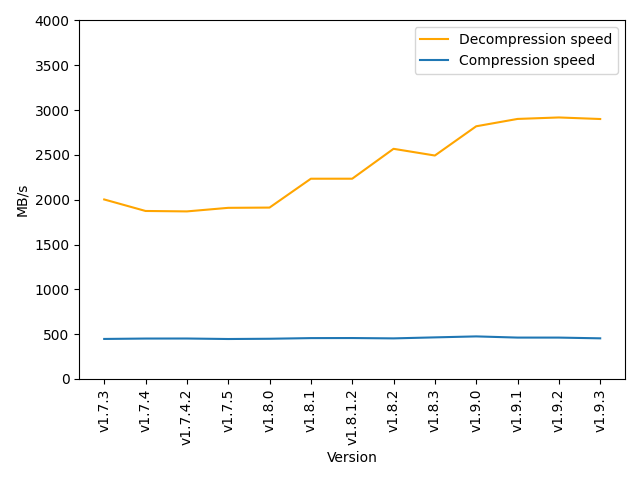
\includegraphics[width=0.8\textwidth]{graph/lz4_releases_plot}
		\caption{Compression- and Decompression speeds throughout the release history}
		\label{fig:release-bench}
	\end{figure}

	As described in the previous section the benchmark was first performed on all versioned releases in the Git repository. The results of this initial run are shown in \autoref{fig:release-bench}. It can be observed that throughout the release history the compression speed stayed relatively consistent. For the decompression speed however, multiple performance increases can be observed throughout the release history. 

	Based on these results the commit range between \textit{v1.8.1} and \textit{v1.8.2} was selected as the commit range for a more thorough and detailed analysis. The results of this analysis are further discussed in \autoref{sec:exp_evaluation}. However as the data for the lz4 benchmark only indicated a performance improvement and the goal of this work is to evaluate the detection both performance improvements and regressions, the release benchmarks were repeated with the \texttt{lz4hc} compression algorithm. The \texttt{lz4hc} implementation is a variant of the \texttt{lz4} implementation that features a higher compression rate at the cost of lower compression speed. As \texttt{lz4hc} is also included in the same source code as \texttt{lz4} the only adaption required to the benchmark was to replace the compression algorithm used in the command line parameters passed.

	\begin{figure}[ht!]
		\centering
		\begin{subfigure}[b]{0.45\textwidth}
			\centering
			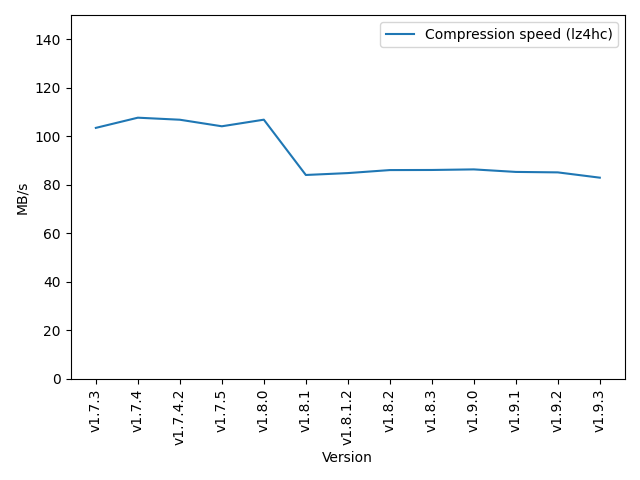
\includegraphics[width=\textwidth]{graph/lz4hc_release_compression}
			\caption{Compression speed of \texttt{lz4hc} releases}
		\end{subfigure}
		\begin{subfigure}[b]{0.45\textwidth}
			\centering
			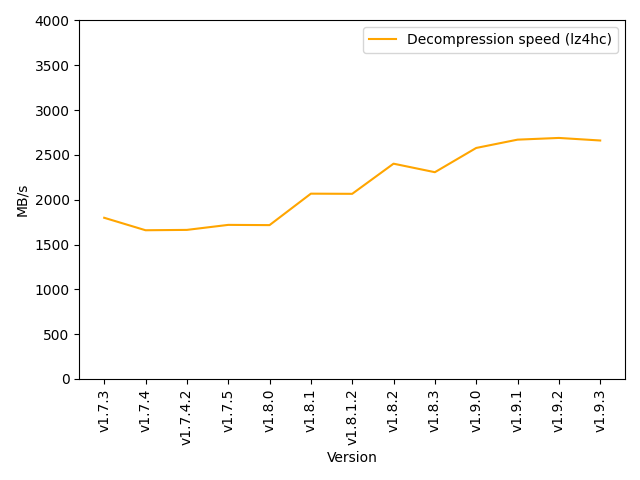
\includegraphics[width=\textwidth]{graph/lz4hc_release_decompression}
			\caption{Decompression speed of \texttt{lz4hc} releases}
		\end{subfigure}
		\caption{Compression and Decompression speeds of \texttt{lz4hc} releases}
		\label{fig:release-bench-lz4hc}
	\end{figure}

	While the graph for the decompression speed is similar to the one for the normal \texttt{lz4} algorithm, for the compression speed a significant performance regression can be observed between versions \textit{v1.8.0} and \textit{v1.8.1}. Therefore this commit range was also selected for further investigation of the individual commits.

\section{Evaluation of Commit Benchmark Results}
\label{sec:exp_evaluation}
This chapter will cover a more thorough analysis of the performance benchmark performed on the identified commit ranges in the previous chapter. Specifically it will compare three algorithms that can be used to detect performance changes and tries to evaluate them. 


\subsection{Reviewing the Performance Benchmark Data}
Before applying automated analysis methods to the data gathered, a manual evaluation of the data gathered from the performance benchmark was conducted. The data gathered for the decompression speed from the \texttt{lz4} benchmark is shown in \autoref{fig:lz4_commit_bench}, while the compression speed data gathered from from the \texttt{lz4hc} benchmark can be seen in \autoref{fig:lz4hc_commit_bench}.

\begin{figure}[ht!]
	\centering
	\begin{subfigure}[b]{0.45\textwidth}
		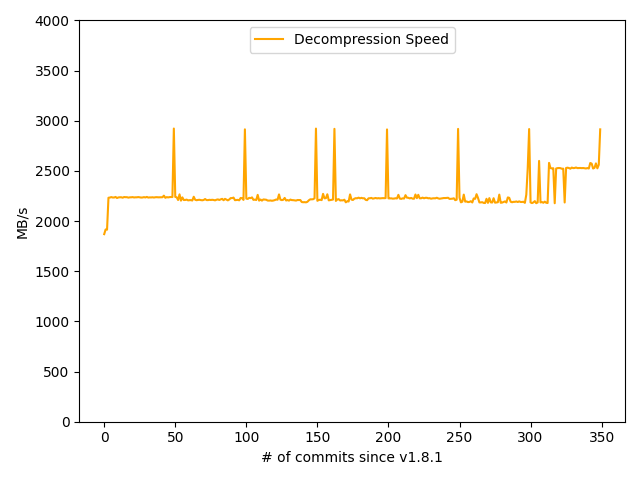
\includegraphics[width=\textwidth]{graph/lz4_commits_decompression}
		\caption{Decompression speed of \texttt{lz4}}
		\label{fig:lz4_commit_bench}
	\end{subfigure}
	\begin{subfigure}[b]{0.45\textwidth}
		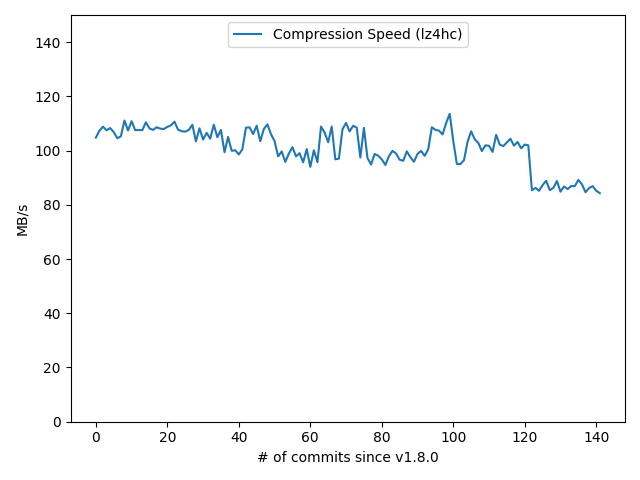
\includegraphics[width=\textwidth]{graph/lz4hc_commits_compression}
		\caption{Decompression speed of \texttt{lz4hc}}
		\label{fig:lz4hc_commit_bench}
	\end{subfigure}
	\caption{Benchmark results for individual commits}
\end{figure}

For the analysis of \texttt{lz4} data there are a few key observation that we made while evaluating the data manually. First of all, it seems that there are at least two general "performance levels" that can be observed from the data: While the majority of the data lies around a speed of 2200 MB/s in the end we see a clear improvement to a level of around 2400 MB/s. We also see that at the very beginning and near the end two more steep increases can be oberseved. However as we are missing the data before and after these benchmarks we cannot rule them out to just be outliers in the dataset. Therefore we do not consider these as additional performance levels.

Another observation that we made were the intense performance increases that can be observed throughout the data series that peak to around 2900 MB/s. While manually reviewing the code changes in the corresponding code commits we could not find any connection to the code changes made that would cause such a spike in the decompression speed nor did we find any evidence of changes being reverted in the following commits that would cause the performance to return to the previous level. This observation will be further discussed in \autoref{ssec:refl_quality} and \autoref{ssec:refl_shortcomings}.

For the data observed for the \texttt{lz4hc} benchmark the data observed does not draw such a clear picture as for the \texttt{lz4} one. From our perspective only one clear change point can be directly observed for the performance drop near the end. Before that there is a lot of fluctuation in the data. One can observe a few short plateaus emerging in the performance data before that, however we cannot decide if these are just effects of random noise or actual relevant performance changes.

\subsection{Comparing Methods to Detect Performance Changes}
After manually reviewing the data we performed a programmatic evaluation of the data with three different methods. Apart from the E-Divisive means algorithm that was already discussed in \autoref{ssec:cp_edivisive}, we will use two more algorithms that were also evaluated by Grambow et al. (See \cite{grambow2019}):

\paragraph{Jump Detection}: This approach performs a relative comparison of the benchmarking data from the current commit to the one right before it. If they diverge by more than a defined percentage, the performance change will be flagged. In our evaluation we used a threshold of 5\%.

\paragraph{Trend Detection}: For trend detection we do not compare the current data to the value of the previous commit but rather we compare it to a moving average of the last $b$ commits. Then similarly to jump detection we check the relative change to this and flag this. For our evaluation we used $b=10$ and similar to jump detection a threshold of 5\%.

\begin{table}
	\centering
	\begin{tabular}{|c||c|c|c|}
		\hline
		\textbf{Benchmark}&\textbf{Jump Detection}&\textbf{Trend Detection}&\textbf{E-Divisive Means}
		\\\hline\hline
		\texttt{lz4}&24&27&4
		\\\hline
		\texttt{lz4hc}&23&43&3
		\\\hline
	\end{tabular}
	\caption{Overview of changes detected by the different methods}
	\label{tab:perf_changes}
\end{table}
After applying these techniques we observed that they differ vastly in the amount of supposed performance changes that they detect. In \autoref{tab:perf_changes} we list how many performance changes were detected for each technique, while \autoref{fig:perf_commit_cp} shows a visual representation of the change points in the datasets.


\begin{figure}[ht!]
	\centering
	\begin{subfigure}[b]{0.3\textwidth}
		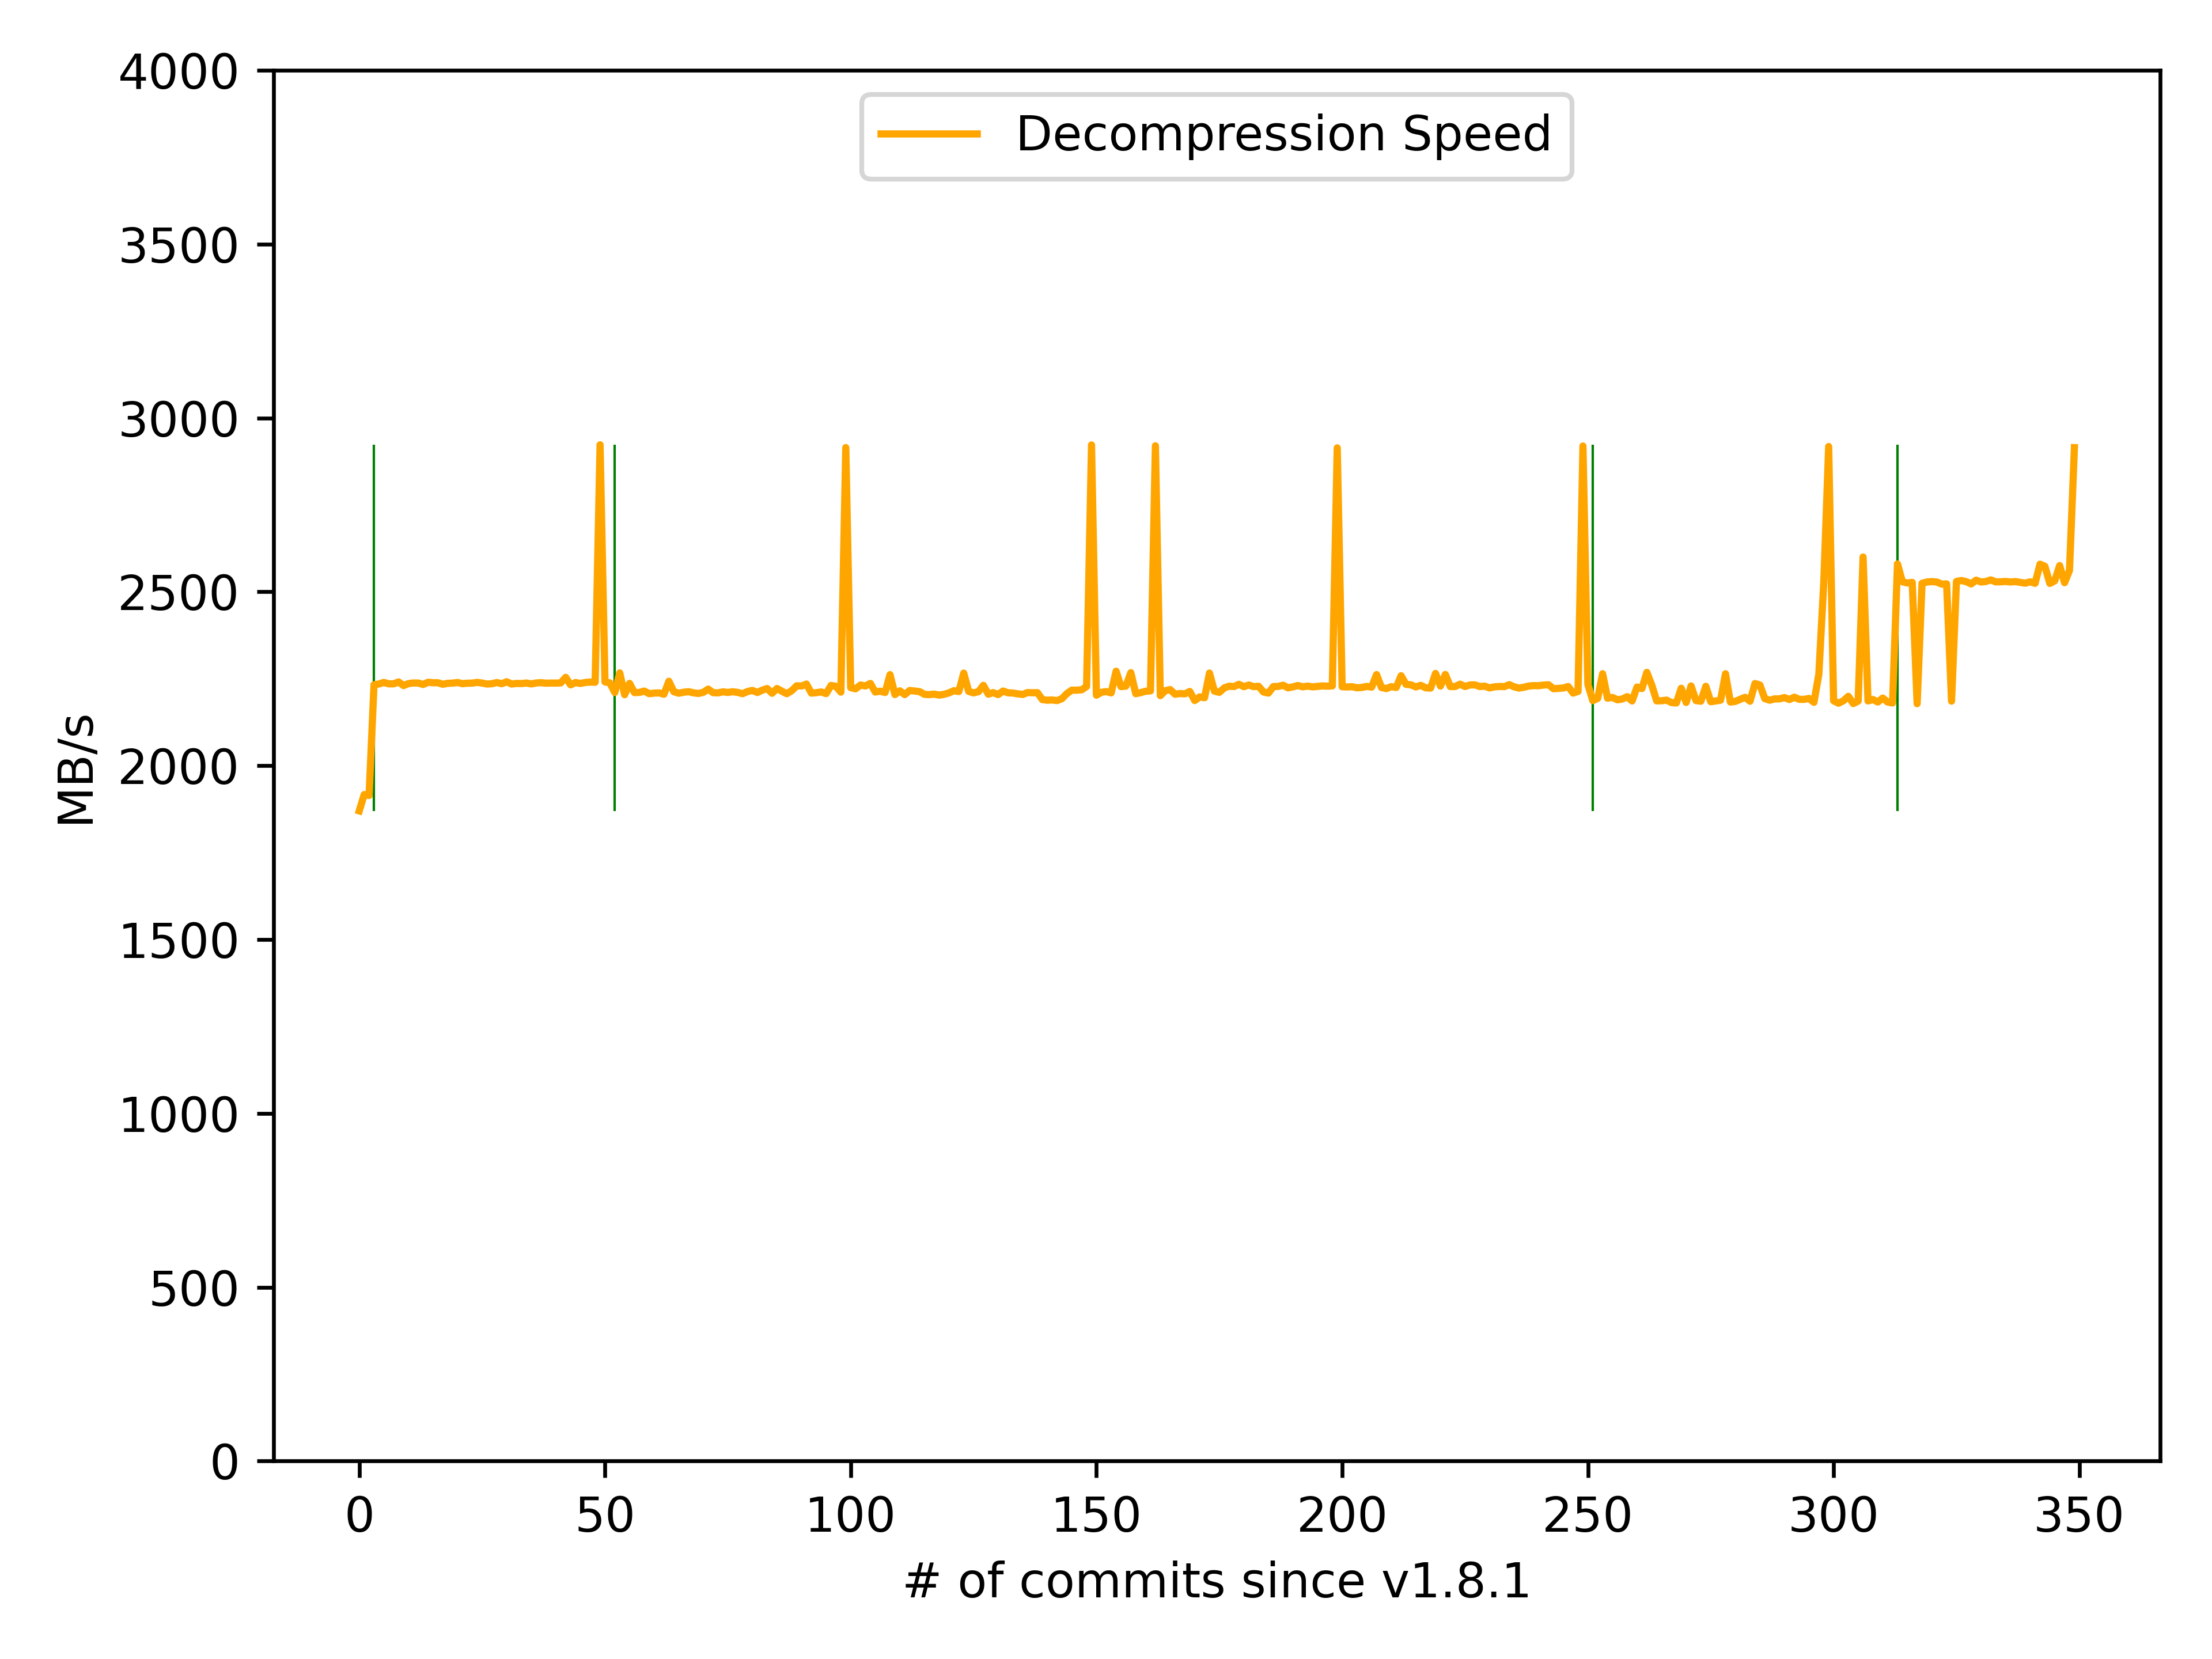
\includegraphics[width=\textwidth]{graph/lz4_commit_e-divisive}
		\caption{\texttt{lz4} using E-Divisive Means}
	\end{subfigure}
	\begin{subfigure}[b]{0.3\textwidth}
		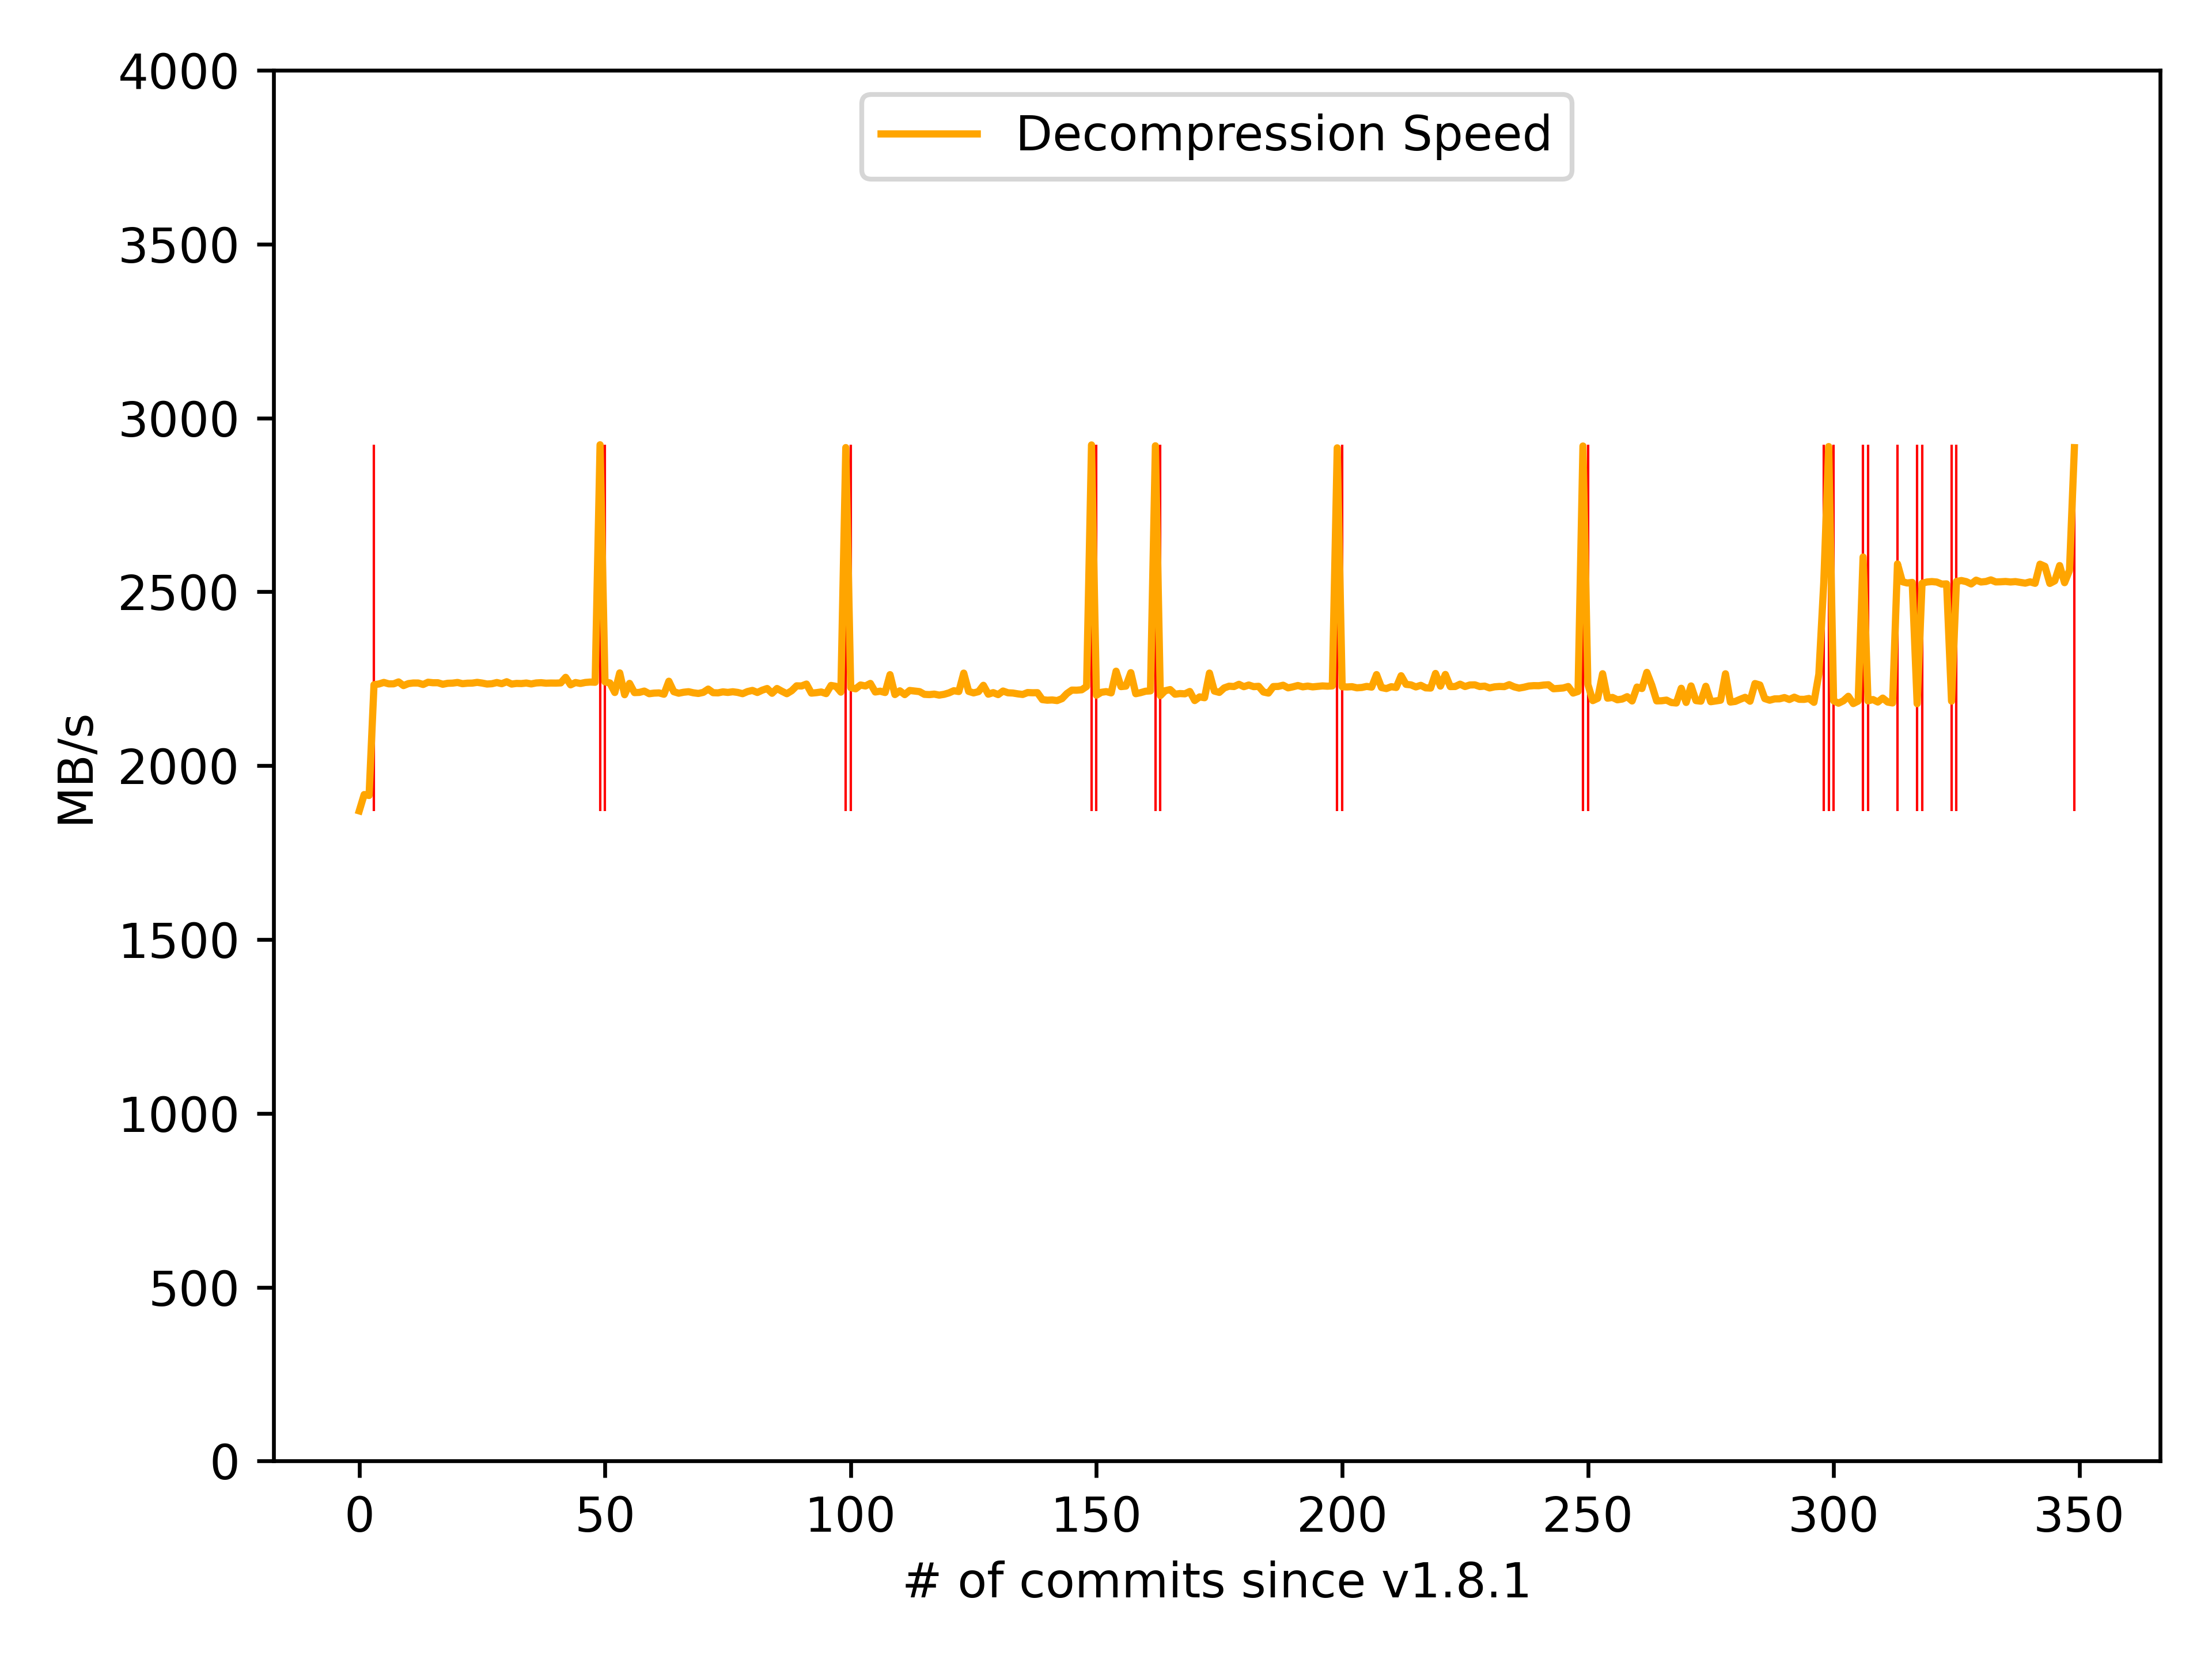
\includegraphics[width=\textwidth]{graph/lz4_commit_jump}
		\caption{\texttt{lz4} using Jump Detection}
	\end{subfigure}
	\begin{subfigure}[b]{0.3\textwidth}
		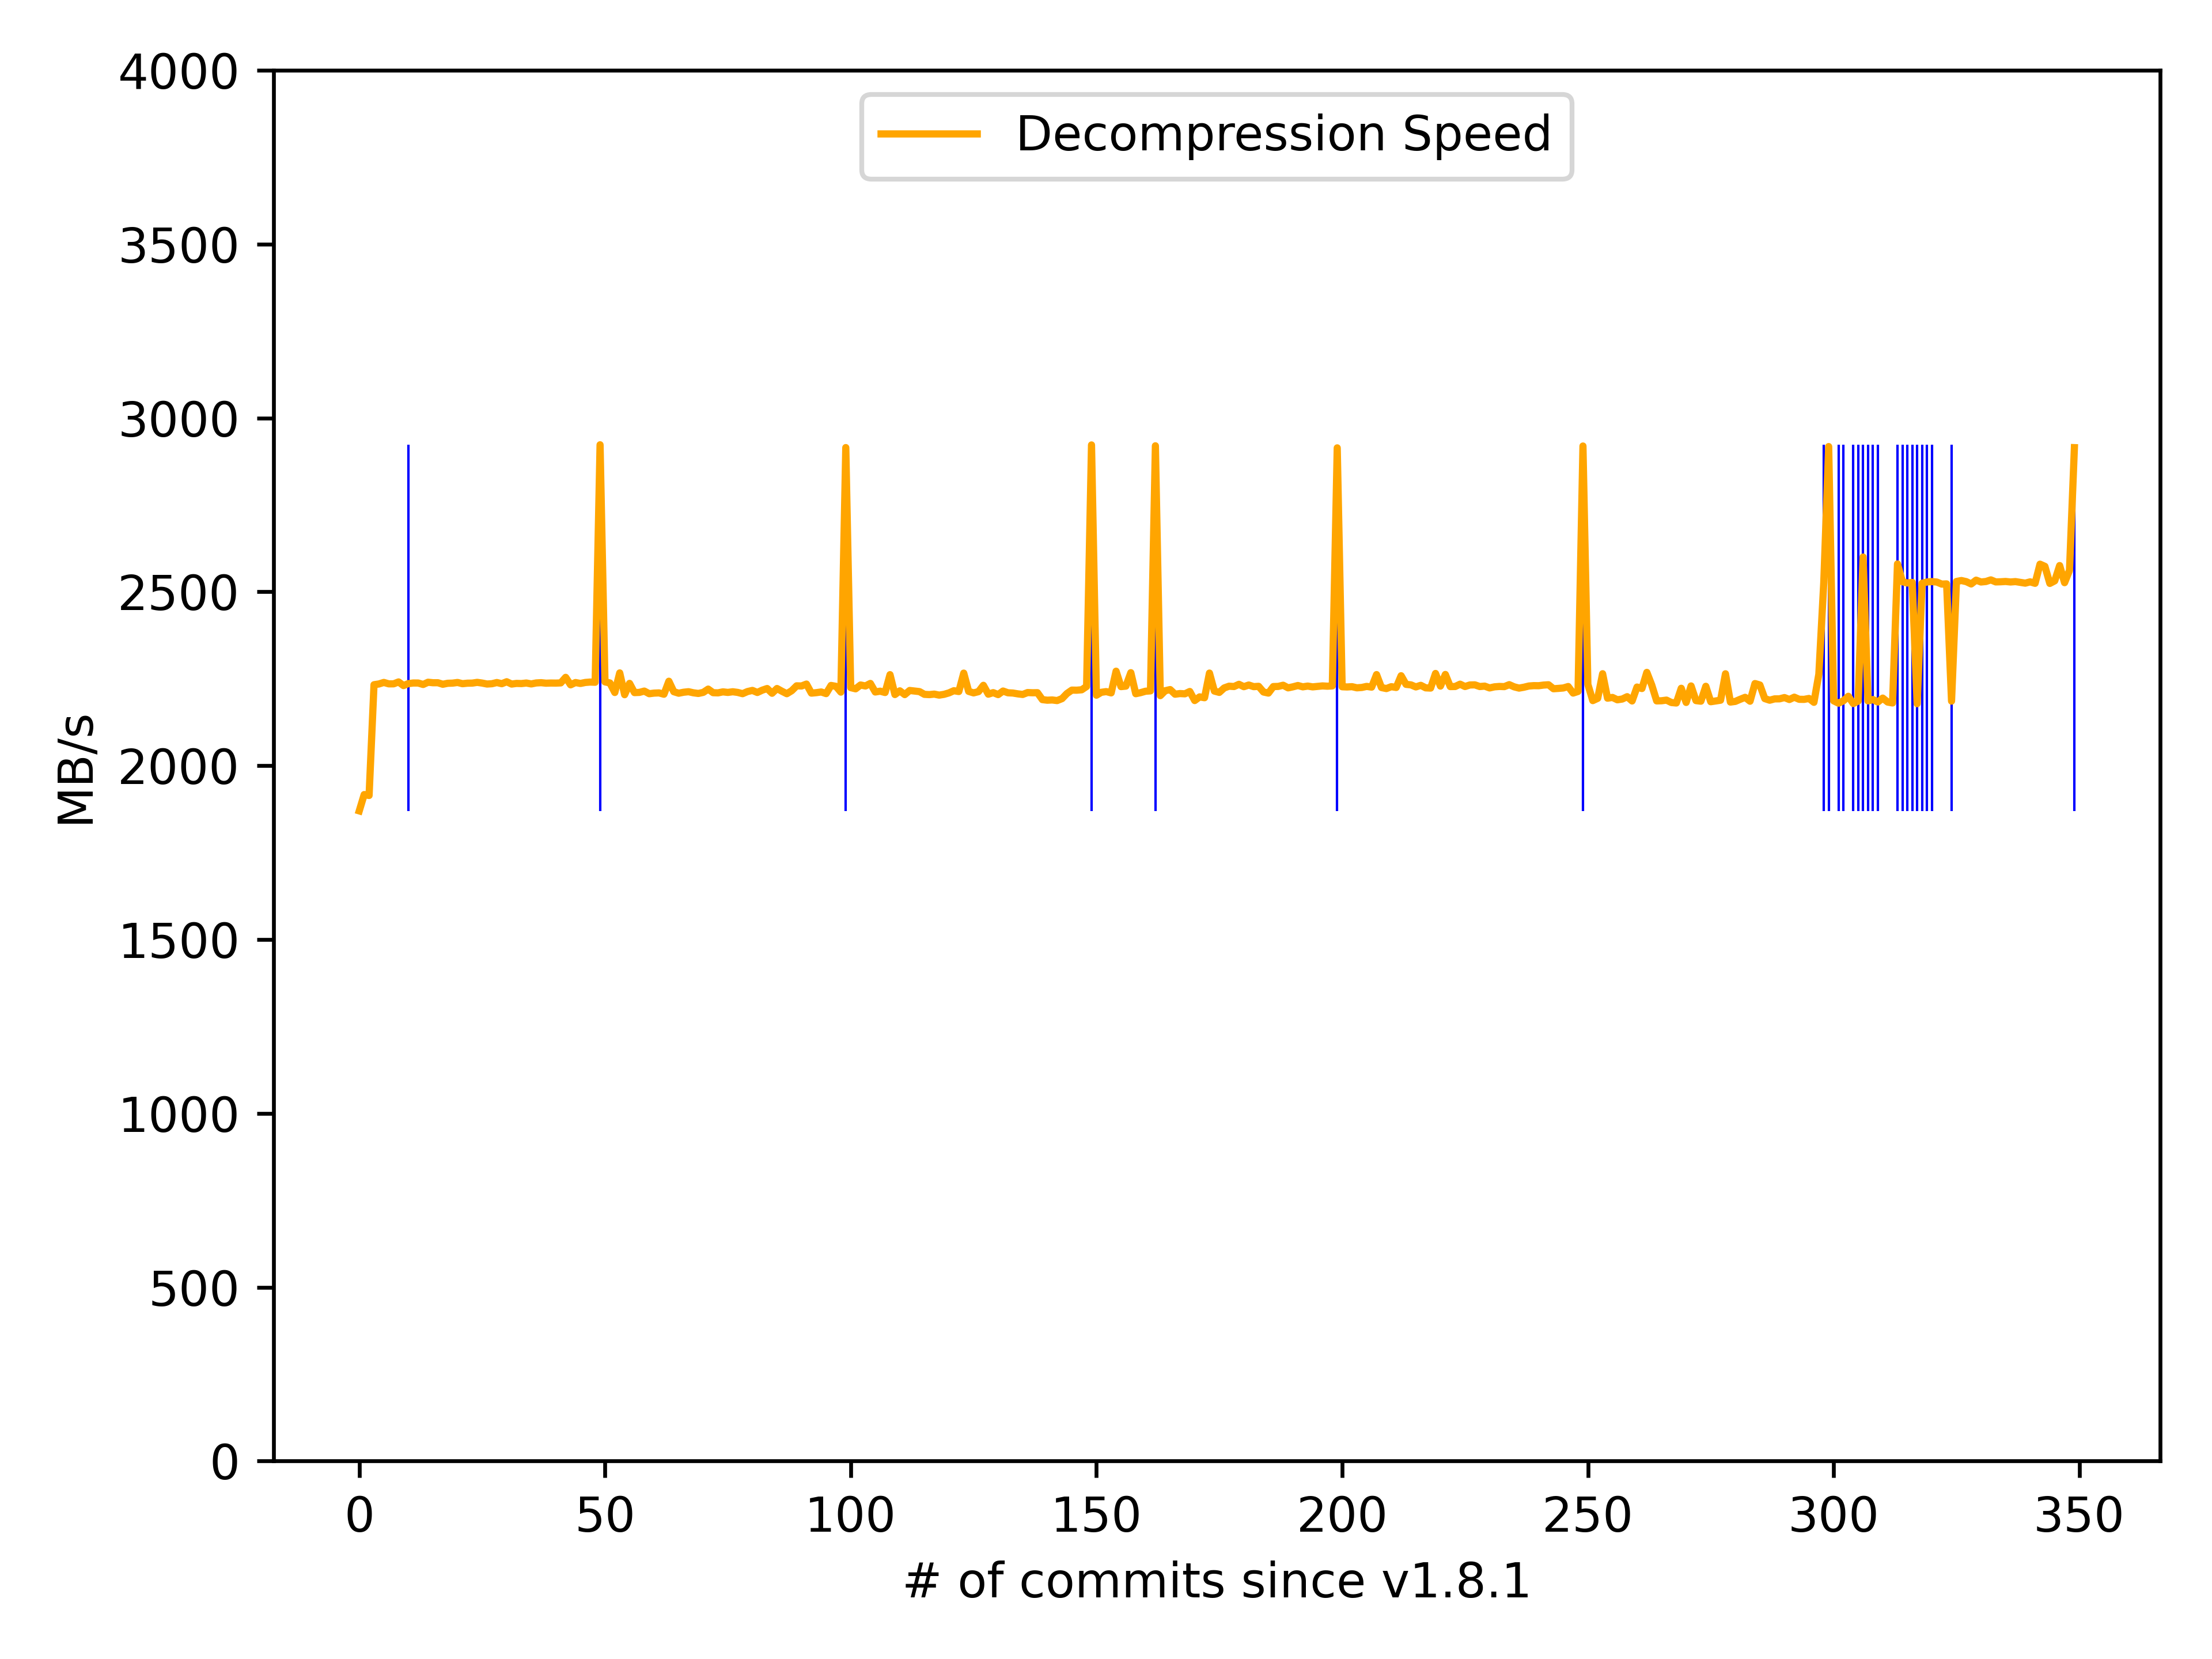
\includegraphics[width=\textwidth]{graph/lz4_commit_trend}
		\caption{\texttt{lz4} using Trend Detection}
	\end{subfigure}
	\begin{subfigure}[b]{0.3\textwidth}
		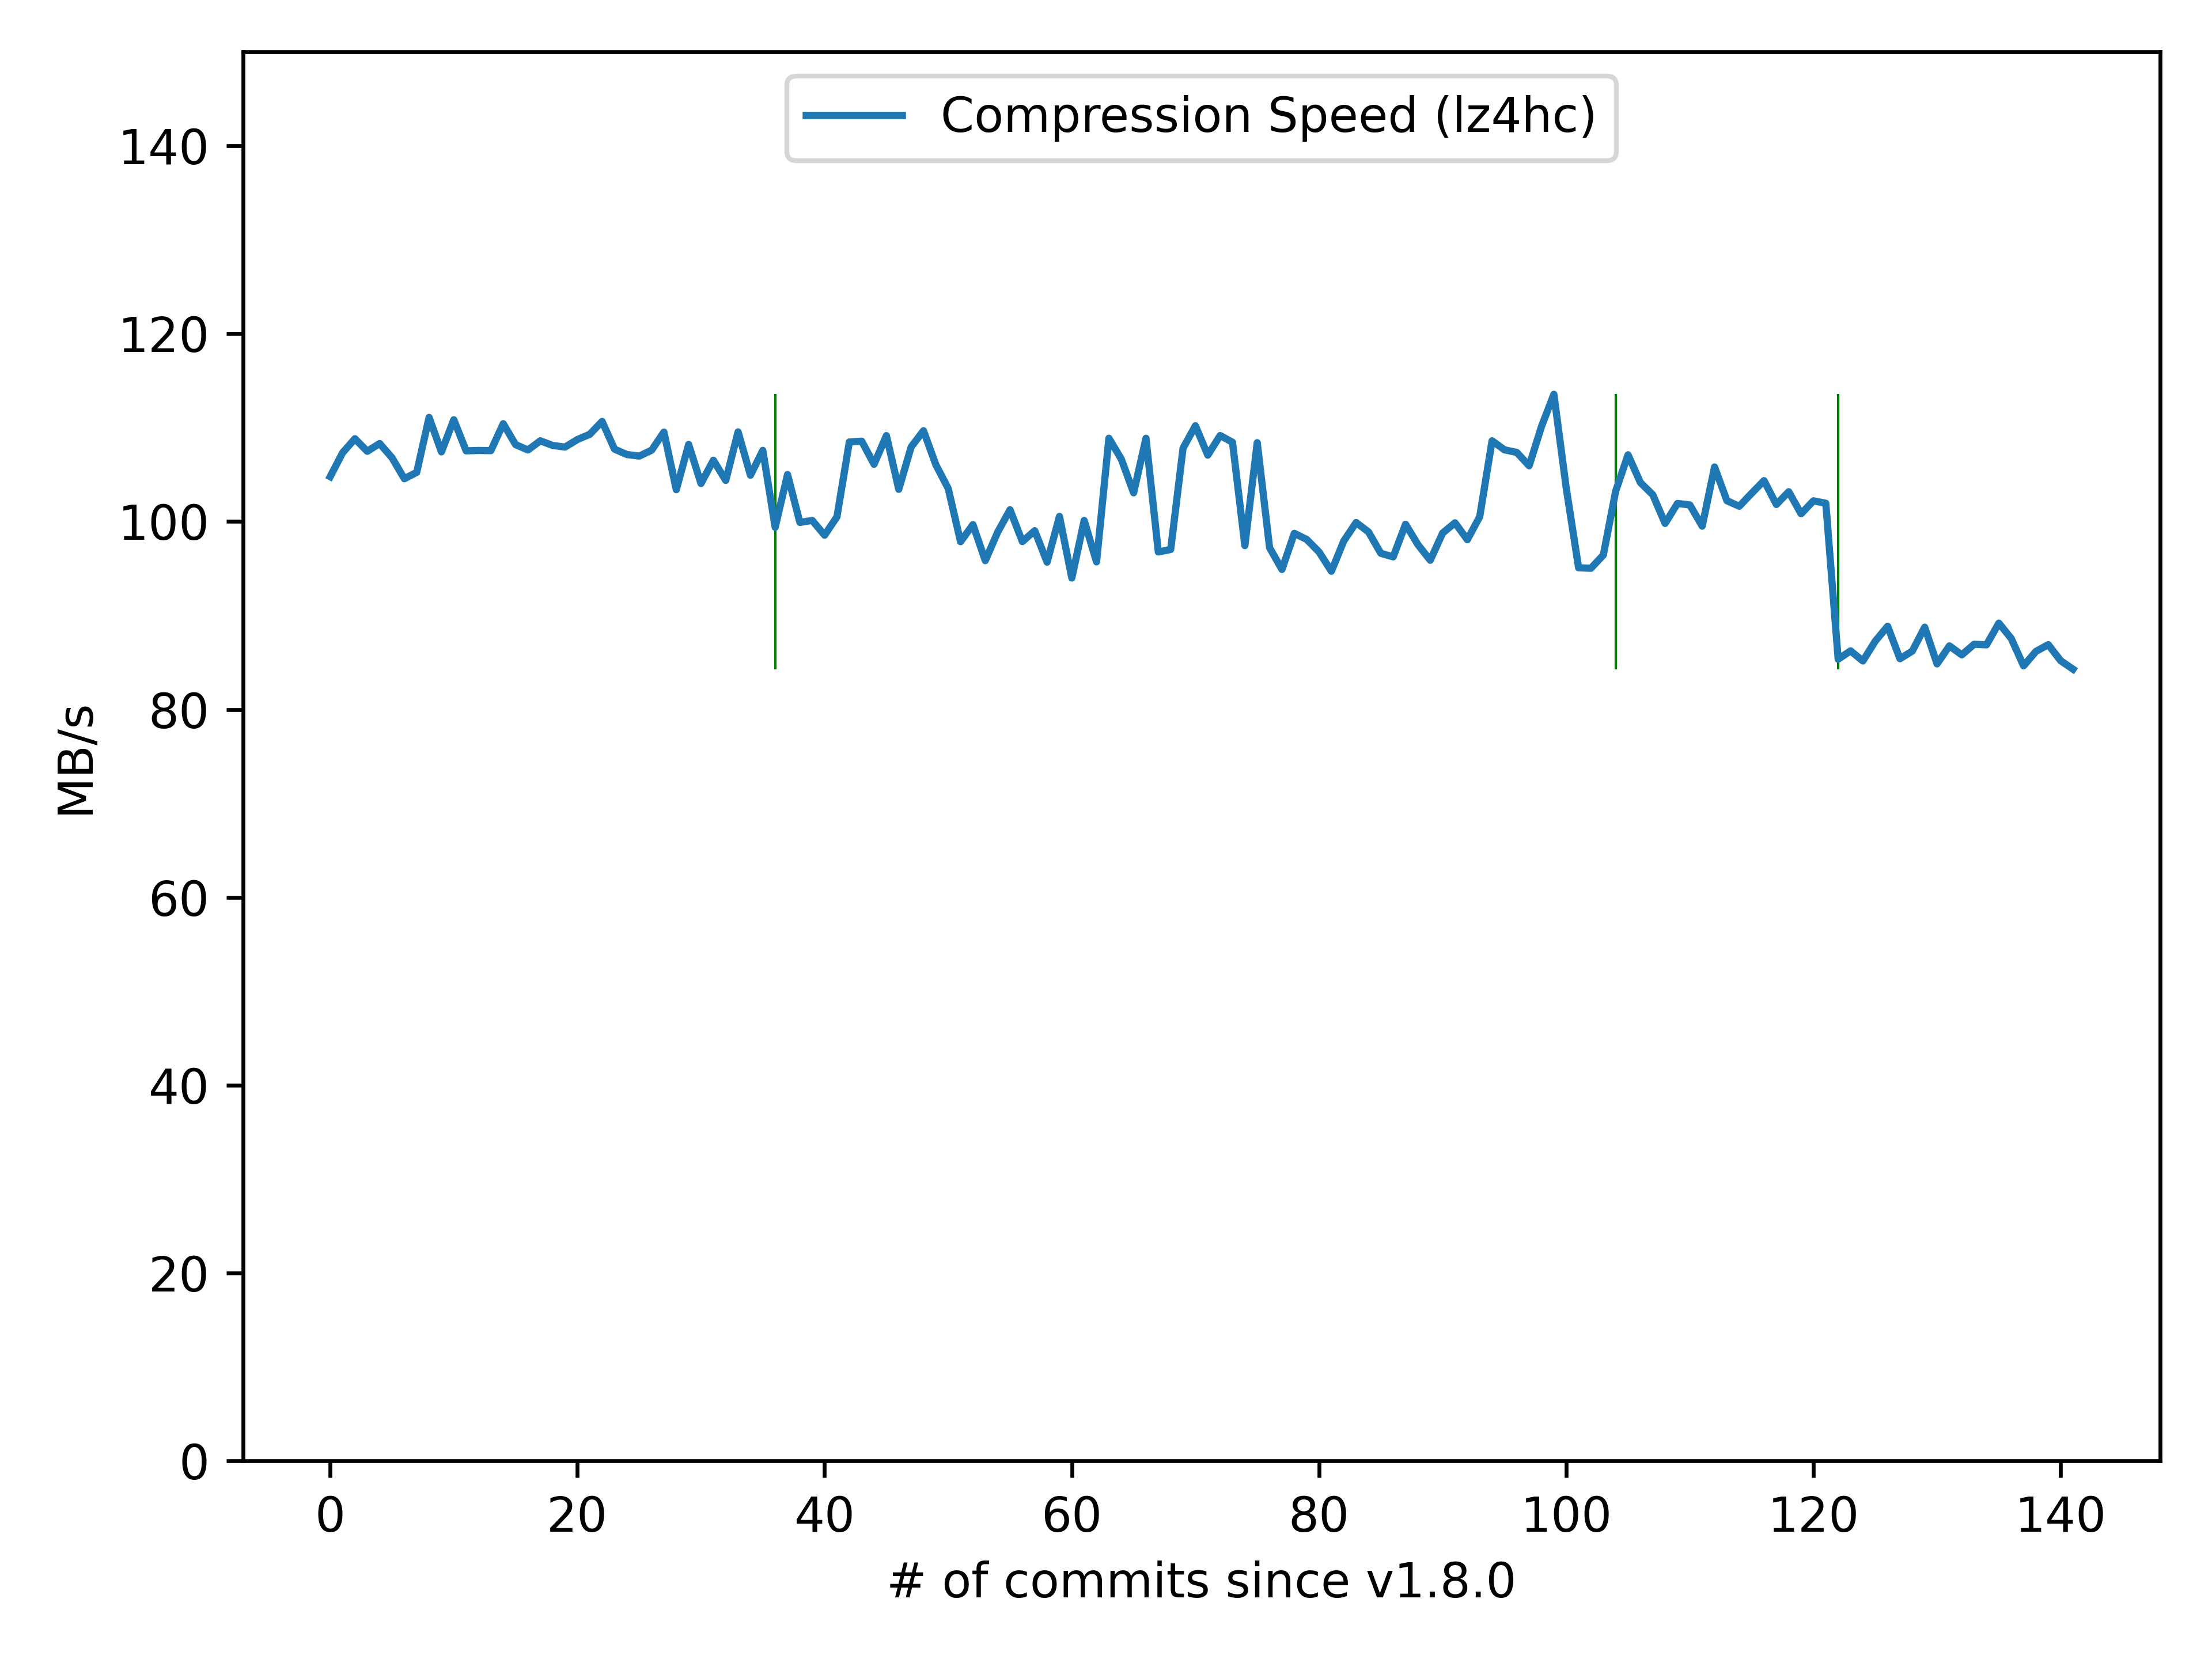
\includegraphics[width=\textwidth]{graph/lz4hc_commit_e-divisive}
		\caption{\texttt{lz4hc} using E-Divisive Means}
	\end{subfigure}
	\begin{subfigure}[b]{0.3\textwidth}
		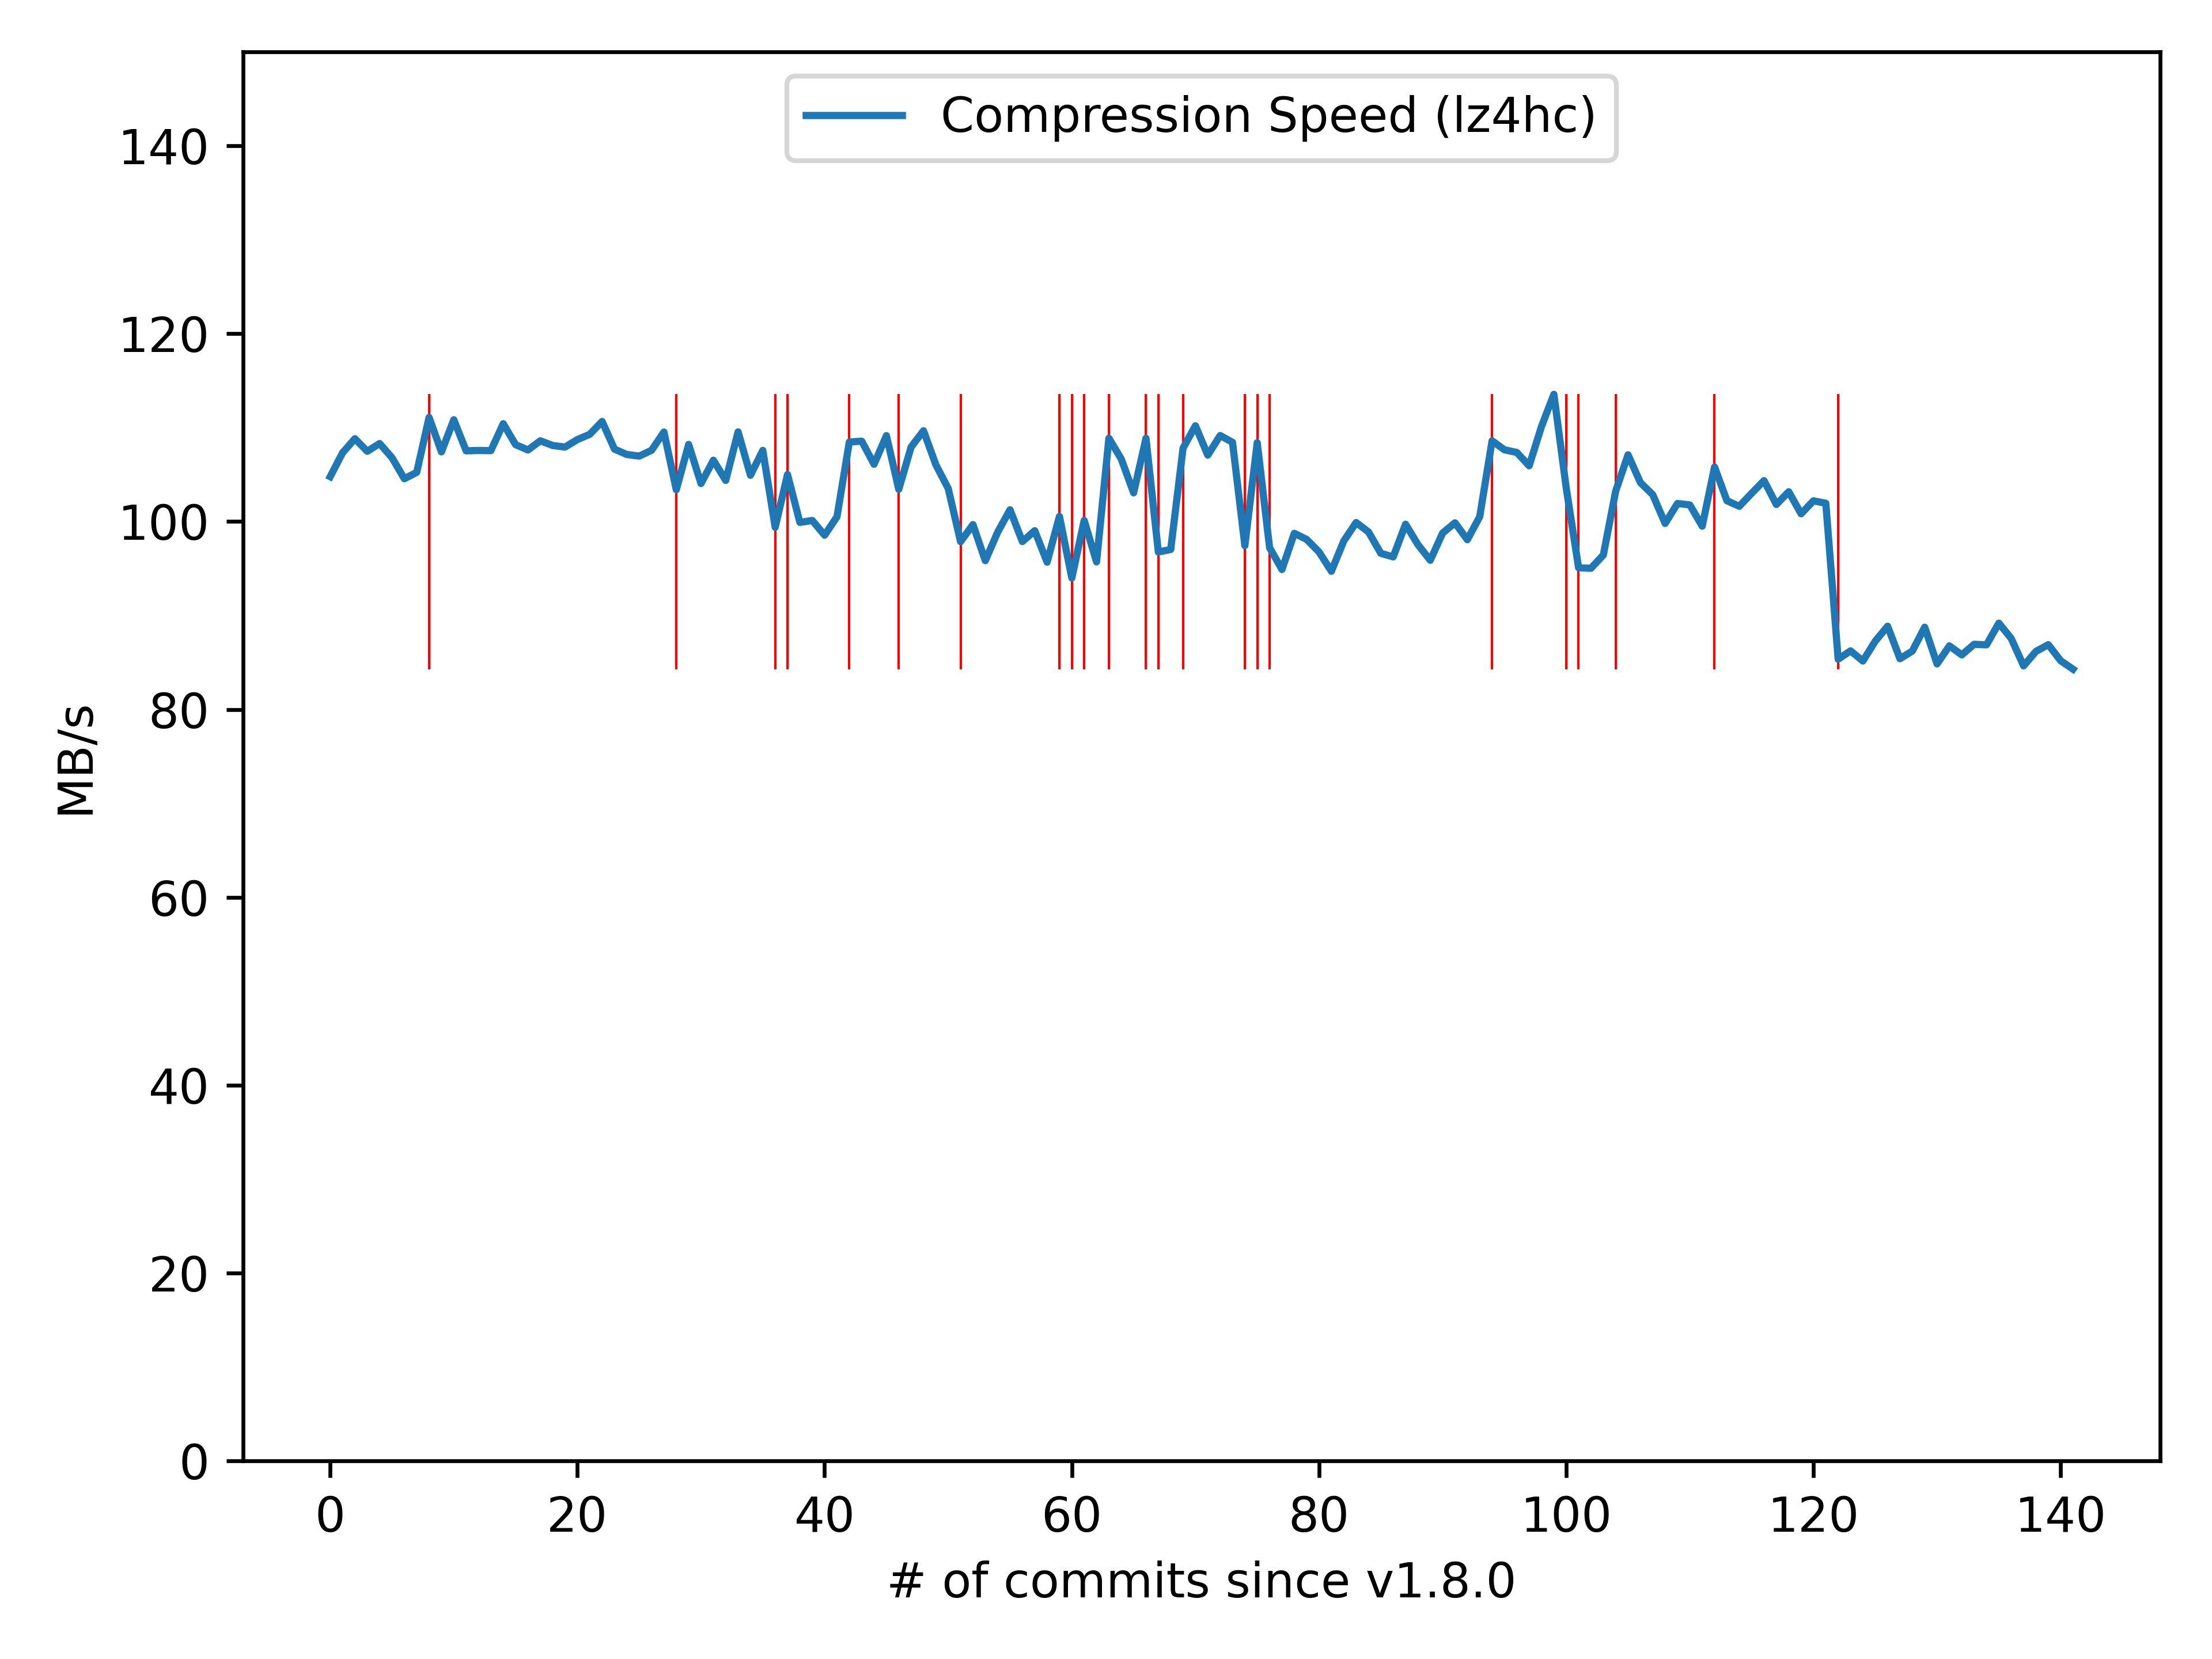
\includegraphics[width=\textwidth]{graph/lz4hc_commit_jump}
		\caption{\texttt{lz4hc} using Jump Detection}
	\end{subfigure}
	\begin{subfigure}[b]{0.3\textwidth}
		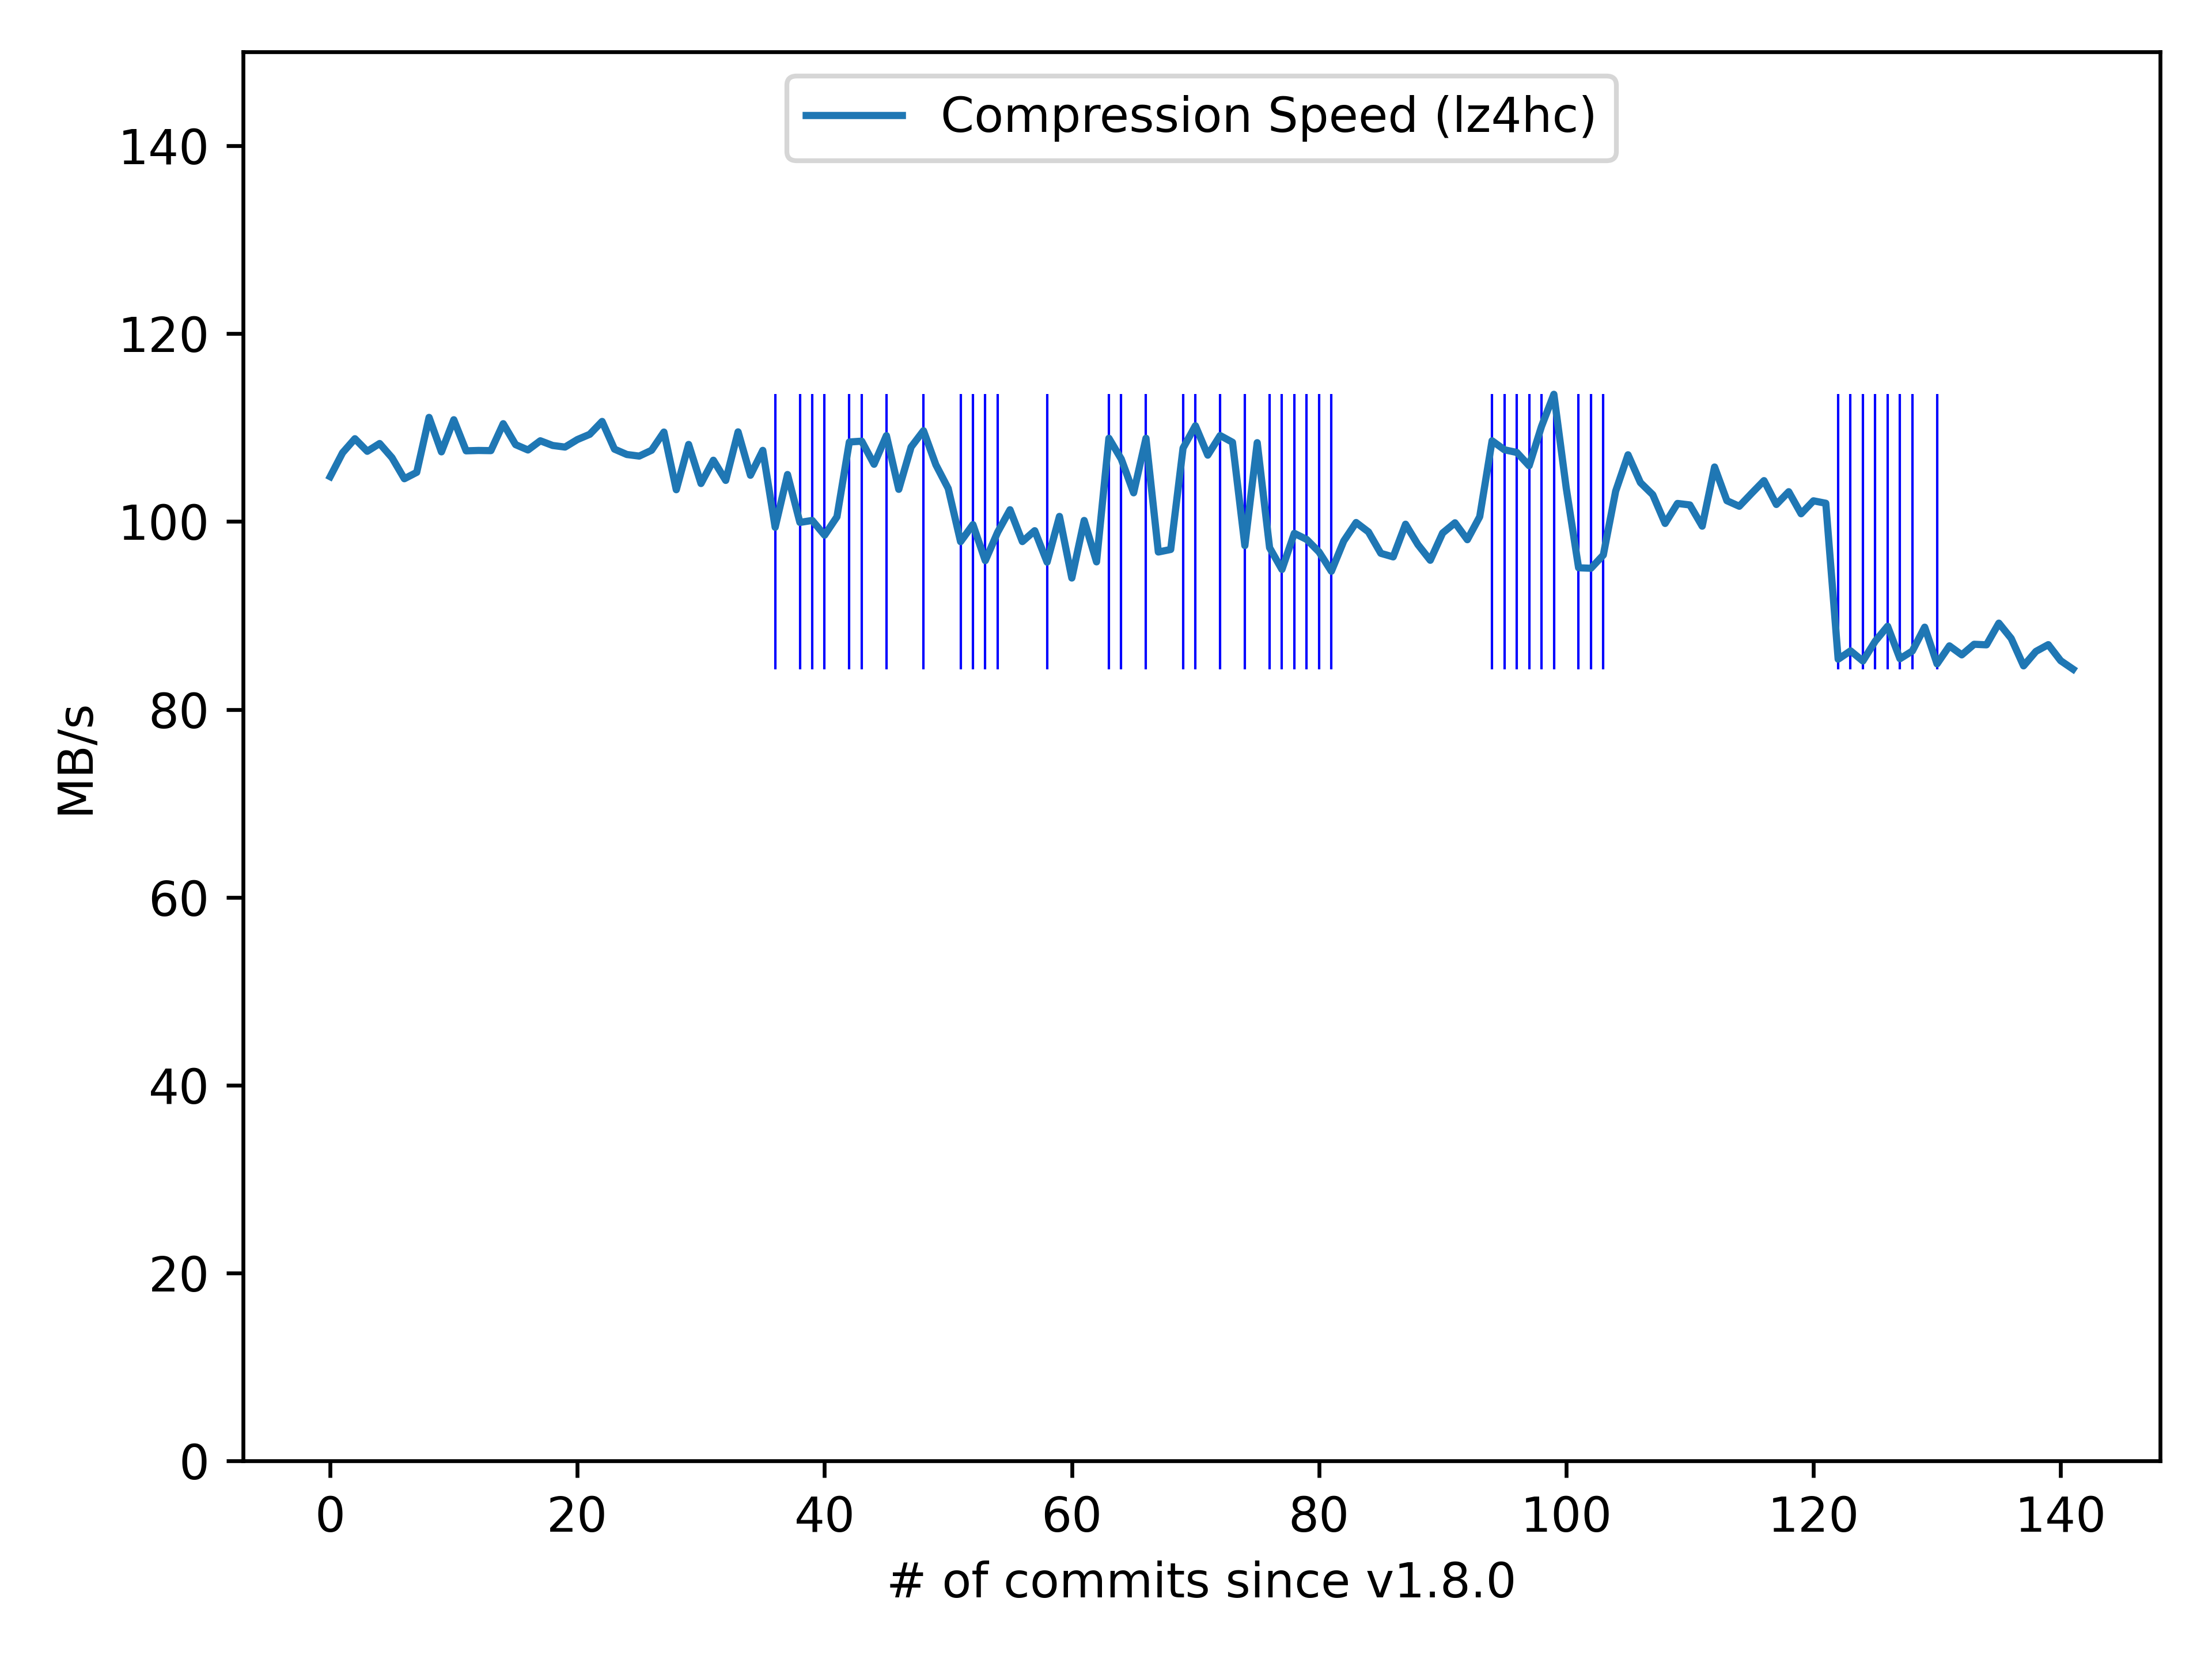
\includegraphics[width=\textwidth]{graph/lz4hc_commit_trend}
		\caption{\texttt{lz4hc} using Trend Detection}
	\end{subfigure}
	\caption{Graphical representation of all change detections on the both datasets}
	\label{fig:perf_commit_cp}
\end{figure}

Surprisingly for us, for both datasets the trend detection flagged the most commits as a performance change. We initially expected that because of the many outliers in our dataset that jump detection would flag the most commits as for every outlier two commits would be flagged -- the outlier and the commit right after that. By far the fewest commits were flagged as changes buy the E-Divisive Means algorithm. To our surprise E-Divisive for the \texttt{lz4} algorithm flagged two additional change points with a relatively small overall performance change that we missed in our manual review. While it is impressive that E-Divisive Mean can detect such changes it is a matter of application domain whether detecting such changes is desirable or if further parameters of the algorithm needs to be tuned.

One more aspect we wanted to evaluate was how quickly these techniques can be detect a performance change after it has occured. While our experiment retroactively looks for change points, we are more interested how and if such techniques can be used to find performance changes while they are introduced.

Intuitively by the nature of Jump Detection it can detect a performance change immediately after it occurs. For trend detection a change can be observed anywhere within the moving average that is given and therefore the detection time depends on the defined parameters.

As E-Divisive means is a different and much more sophisticated change point detection algorithm as the other two evaluating when a change will be detected is not as trivial. However as E-Divisive means specifically only detects change points and not outliers, it will never flag the latest commit as a performance change as this could very well be the result of an outlier.

To evaluate how quickly a performance change is detected by E-Divisive Means, we use the data we gather to retroactively "simulate" an ongoing continuous benchmarking approach. That is we iteratively add one commit by one to the time series and therefore find the first occurence of the change points identified in our final time series. The results of this evaluation are shown in \autoref{tab:ediv_occ}

\begin{table}
	\centering
	\begin{tabular}{|c||c|c|c|}
		\hline
		\textbf{Dataset}&\textbf{Change Point Commit\#}&\textbf{First detected at Commit \#}&\textbf{$\Delta$}
		\\\hline\hline
		\texttt{lz4}&3&7&4
		\\\hline
		\texttt{lz4}&52&64&12
		\\\hline
		\texttt{lz4}&251&287&31
		\\\hline
		\texttt{lz4}&313&316&6
		\\\hline
		\texttt{lz4hc}&36&37&1
		\\\hline
		\texttt{lz4hc}&104&122&18
		\\\hline
		\texttt{lz4hc}&122&123&1
		\\\hline
	\end{tabular}
	\caption{Overview of changes detected by the different methods}
	\label{tab:ediv_occ}
\end{table}

So for our example, E-Divisive Means detects the changes relatively quich in most cases. When reviewing these commits by hand we found that the biggest time difference was about four weeks until the change point got detected (Between commit 104 and 122 for \texttt{lz4hc}). For most of the other change points it was only a few days until the detection. Whether or not a detection time of four weeks is acceptable is heavily project dependent and cannot be answered by us generically.

\subsection{Conclusion}
We believe that all three algorithms presented in this chapter offer useful properties for certain application with respect to detecting performance changes. However when it comes to reliably detecting performance changes throughout the development, we believe that E-Divisive Means stands out against the other two. Jump Detection is neturally prone to noisy signals while for trend detection we observed a fairly poor performance on bi-modal data as we partly oberseved it in our \texttt{lz4} dataset.

However also E-Divisive means has its drawbacks that should be considered before implementing it: For a reliable and vast change detection one needs to regularly benchmark the \gls{sut}, optimally after every code change. In practice this might not be viable. Also we observed that it flags even smaller performance changes which might not desirable. Lastly depending on the performance data it might take some time for the algorithm to identify a change point. However for this last point one needs to consider that E-Divisive Means still identifies the exact point where a performance change was introduced which potentially reduces the amount to find the corresponding code change by far.

\section{Reflection}
In this section the results of this work are critically reflected upon. A focus is put onto the quality of the benchmark experiment ran. Additionally the shortcomings of the approach used will be discussed to identify potential future work that could extend this work.

	\subsection{Quality of the Benchmarking Experiment}
	\label{ssec:refl_quality}
	In this chapter we will focus on the quality of our benchmarking experiment we conducted. We will hereby evaluate each of the five quality attributes that were already mentioned in \autoref{ssec:eval_bm}.

	\paragraph{Relevance} -- We believe that this aspect has to be viewed from two different angles. The first one would be, how relevant the benchmark is in terms of detecting performance changes in the \texttt{lz4} software. In this regard we believe that this benchmark certainly provides a specific relevance as we have shown with different techniques how to retroactively identify performance changes in the software.

	The other aspect however, is how relevant the results of our experiment are to our overarching question: "Should we benchmark software only before releases or after every commit". For this we believe our benchmark has only a limited relevance. The main reason for this is that our experiment only covered a really simplified and streamlined example. For the example of \texttt{lz4} performing a benchmark after every commit might be feasible; However our benchmark did not at all consider the dimension of modern software systems such as configurability which makes this approach unfeasible for most potential use-cases.

\paragraph{Reproducibility} -- As all code artifact that have been used to perform this benchmark have been documented in a GitHub repository. A third-party could use these in addition to the information given in this paper regarding the hardware configuration to closely reproduce the results.

\paragraph{Fairness} -- As for fairness there are a few things to criticise. Our benchmark is completely created artificially and is overly simplistic by nature. Therefore the fairness of our benchmarking approach could be questionable.

\paragraph{Verifiability} -- In terms of verifiability, our benchmark ensures that only a predefined software configuration is used. However our benchmark only copies the build files from an existing directory on the users hardware and does not validate if any unexpected changes have been made. In an extended approach we would rather consider the code to be cloned directly from a public Git repository, preferably with a specific commit defined.

Additionally our detailed experiment contained some outliers that we could not explain based on our findings. We now believe that this might be an error in our benchmarking approach as firstly, the achieved performance results are closely to those from recent \texttt{lz4} versions. Additionally when repeating the benchmark on a smaller subset, we could not reliably reproduce these results. Unfortunately in the time frame of this seminar we could not identify the exact cause of this.

\paragraph{Usability} -- In terms of usability, we believe that our benchmark is, at most to a certain extent, quite usable. While we used a compute cluster to run multiple benchmarks in parallel we believe that comparable results could also be reproduced by just using one local machine.

	\subsection{Shortcomings}
	\label{ssec:refl_shortcomings}
	There are several shortcomings of our experiment that can be discussed. First of all we have already discussed that there were some inconsistencies in the data gathered from the experiment. This has caused some, otherwise unexplainable, performance spikes in the data. As we could not reliably reproduce this behavior we believe that there is some issue in our benchmarking pipeline which leads to a wrong version of \texttt{lz4} being used. Therefore, one could argue that it cannot be out ruled that also other data recorded is not flawed in some other unnoticed way.

	Secondly while we have retroactively identified change points using our methodology we have not performed any verification on these. Optimally we should have verified if the change points we identified are actually related to code changes by manually reviewing the corresponding commits in the Git history. This was not done in the scope of this paper due to the limited time available.

	Thirdly our benchmark experiment itself was too simplistic in nature. It gives a broad first overview however we believe that it is generally not transferable to the development of complex software systems.

	\subsection{Future Work}

	To react and further evaluate on the shortcomings identified there are several opportunities for future works that could extend this paper. Most significantly we should focus on fixing the benchmark suite itself such that we can verify the correctness of the data produced.

	Secondly we believe that for future works the focus of the research question should shift a bit. While this work shows that in an optimal scenario one should benchmark every commit, this is not applicable in practice. Therefore the focus should rather shift to find strategies to preemptively select the "correct" commits for benchmarking.

	Lastly we believe that that aspect of configurability needs to be further considered. While we already collected data for two variants of \texttt{lz4}, we did not use it yet to find any collaborations between the data. We believe that exploring possibilities to link performance changes across variants can be very beneficial.

\section{Related Work}

Several similar work has been published regarding continuous performance benchmarking. Both Antz et al. and Waller at al. describe methods how benchmarking can be included into a continuous integration pipeline to enable continuous benchmarking(\cite{antz2019}, \cite{waller2015}). Additionally Daly describes in multiple works how a continuous benchmarking approach has been introduced to MongoDB to enable better detection of performance changes(\cite{daly2020}, \cite{daly2021}).

In the domain of identifying performance changes across different software configurations and variants, Apel et al. present a novel change point detection algorithm that can identify configuration-dependent performance changes while only exploring a small subset of the configuration space (\cite{apel2020}).

Multiple works have also been presented to predict performance changes in software based in order to reduce the amount of commits that need to be benchmarked. One of these approaches is \textit{Perphecy} presented by Oliveria et al. (\cite{oliveira2017}). Similarly, Chen et al. present an approach which identifies which predicts which test cases may suffer from performance regressions after a code change(\cite{chen2020}).

\section{Conclusion}

In this paper we tried to answer the question whether one should benchmark software only before releases or after every commit. We have explored both possibilities and compared different performance change detection methods. We come to the conclusion that, in an optimal scenario, benchmarking every commit would be the preferable option.

However we also want to highlight that this paper is based on data from a overly simplistic benchmark and suffers from several shortcomings. Therefore the applicability to productive systems is limited and for most real world systems benchmarking every commit is simply not feasible.

We therefore highlight that further work is required to sufficiently answer the question. Most notably it needs to be explored in which ways the overall number of commits and configurations to benchmark can be reduced while still reliably detecting performance changes.
	
	%*********************************************************************%
	% APPENDIX                                                            %
	%*********************************************************************%
	
	% Insert the appendix here. You can alternatively include files via: \include{pathToFile}
	
	%*********************************************************************%
	% LITERATURE                                                          %
	%*********************************************************************%
	% As a recommendation JabRef might be a usefull tool for this section. Use myRefs.bib therefore
	\phantomsection
	\bibliographystyle{splncs03}
	\bibliography{literature}
\end{document}
